This chapter gives the experimental details behind this thesis. The work here combines two major fields, THz spectroscopy and compressed sensing. Whilst nothing new is presented in regards to each individual field, the novelty is the successful combination of the two. The first two sections summarize THz spectroscopy and the latter two describe how one can perform compressed sensing in a THz time-domain spectrometer.   


\section{THz Time domain spectrometer}\label{sec:THz_TDS}
The fundamental layout of the setup is shown in figure \ref{fig:THz_TDS}. In its essence, a beam of femtosecond optical pulses is split into three beams: generation, detection and excitation. The first is used to generate a picosecond THz pulse, through optical rectification in ZnTe as discussed in sec. \ref{sec:THz_gen}, which then passes through the sample under investigation. Our THz beam is collimated and collected by 90$^\circ$ off-axis parabolic mirrors made from gold. The second beam is used to detect the time profile of the THz waveform. This is achieved by temporally overlapping the much longer THz pulse with the very short detection pulse. The difference in pulse durations allows one to discretely sample the terahertz temporal profile by varying the path lengths with an optical delay line (typical THz transient and detection pulse envelope shown in figure \ref{fig:THz_pulse}). The electric field amplitude is extracted via electro-optic sampling in a ZnTe crystal, discussed in sec. \ref{sec:THz_det}. These systems detect the amplitude and relative phase of the THz pulse. This allows for the extraction of a real and imaginary permittivity of a sample as discussed in sec. \ref{sec:extract_perm}. The third beam is used to photoexcite the sample. These three beams are what constitute a typical THZ-TDS system. However, additionally in our system, the excitation beam is spatially modulated via a digital micromirror device (DMD) and a lens so as to project any binary intensity pattern onto our sample. Further more, our DMD is synchronized to the main laser system. The reason for this is discussed in sec. \ref{sec:had_mat}.
\begin{figure}[h!]\centering
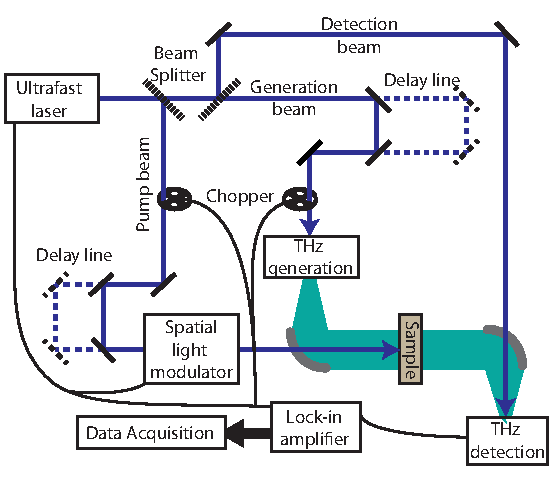
\includegraphics[width=0.73\linewidth]{Chapters/Experimental/THz_TDS.pdf}
\caption{\textbf{Schematic of time domain terahertz
spectrometer.} A beam of ultrashort optical pulses leave an ultrafast laser. The beam is split into three beams: generation, detection and
excitation. A chopper is placed in the detection or generation beams,
depending on the needs of the experiment. A spatial light modulator, which can be synchronized to the ultrafast-laser, is placed in the excitation beam. Parabolic mirrors are used to collect and collimate the THz radiation.}
\label{fig:THz_TDS}
\end{figure}

\subsubsection{The ultra-fast laser source}
The starting point of our THz-TDS is the laser powering the entire setup; a Ti:Sapphire system consisting of a seed laser and and regenerative amplification stage. Titanium-doped sapphire crystals have an absorption peak at 520$nm$ and exhibit a gain over a large wavelength range, from 650$nm$ to 1100$nm$, with a maximum at 800$nm$ (see ch. 3.1.2 of ref. \cite{PrinciplesofTHz}). Further, these crystals can withstand large optical pump power ($\sim 20W$). In our seed system, \textit{Coherent Vitesse},  the Ti:Sapphire crystal is pumped using a 535$nm$ diode laser. The excited electrons within the crystal relax down to a lower state and emit photons with central wavelength 800$nm$. The continuous wave emission is converted in to pulses via a Kerr-lens modelocking mechanism. The emitted pulses have a duration of 85$fs$, 12$nJ$ of energy per pulse and a repetition rate of 80$MHz$. 

However, for the non-linear optical phenomena used to generate THz radiation in this thesis (\S \ref{sec:THz_gen}) to be efficient, much bigger pulse energies are needed.  Further more, most experiments here photoexcite a silicon wafer in order to modulate our THz pulse, see \S\ref{sec:THz_mod}, which also requires large pulse energies. This is why we have a regenerative amplifier, \textit{Coherent Legend Elite}, to increase the energy of the seed pulses although at lower the repetition rate. Before amplification, the seed pulses are temporally stretched using a reflection grating and collimating optics. This stretching stage lowers the instantaneous pulse intensity and thus avoids damaging the energy amplification optics at later stages. The regenerative amplifier is another Ti:Sapphire laser cavity that is optically isolated from the seed laser. The gain medium is pumped with its own diode laser until it has sufficient amounts of energy to be used an amplifier for the seed pulses. Unfortunately, this waiting stage results in throwing away many of the pulses from the seed laser. The seed pulses are injected into this amplification cavity with a Pockels cell and a polarizer\footnote{When the Pockels cell is biased with a voltage it changes the polarization of the pulse so that it is transmitted by the polarizer.}. The injected pulses absorb the energy in the gain medium increasing their own field strength every time they make a round trip in the laser cavity. This process carries on for approximately 20 round-trips until the pulses are switched out of the cavity with a second Pockels cell. Then the temporal stretching stage is reversed using another grating in order to compress the amplified pulses in to a 100 femtoseconds. In the end this amplification stage results in an increase in the instantaneous pulse intensity by a factor of $2 \times 10^6$ and a decrease in repetition rate by a factor of $8\times 10^4$. The amplifier output is a train of pulses with temporal length of 100$fs$, 3$mJ$ energy per pulse, 800$nm$ central wavelength and a repetition rate of 1050$Hz$. 


%--------------------------------------------------%
%----%----%----%---- THZ  Pulses ----%---%----%----%
%--------------------------------------------------%
\subsection{Single-cycle THz transients} %Moved this section near the start of the chapter
\begin{figure}[h!]\centering
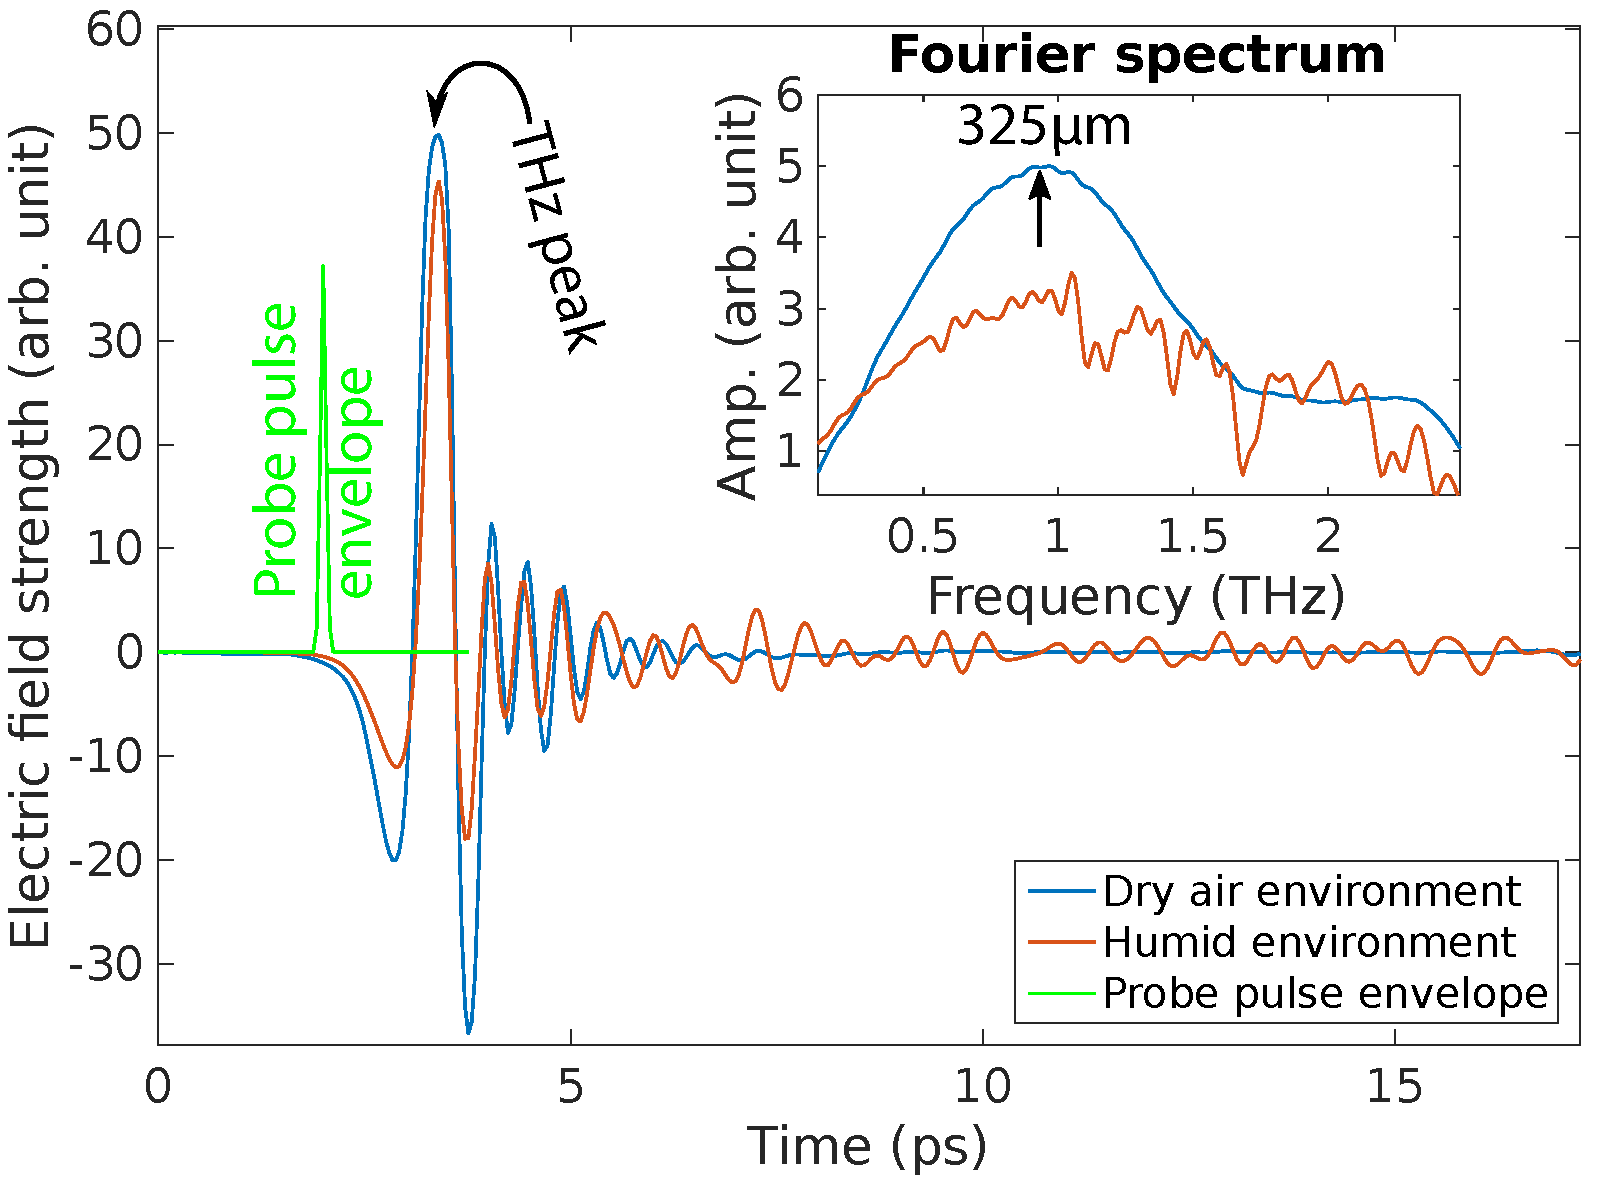
\includegraphics[width=0.71\linewidth]{Chapters/Experimental/THz_pulse.pdf} %Updated this figure
\caption{Red: typical THz pulse detected by our system in normal room conditions (\~35\% humidity). Blue: THz pulse recorded in a box pressurized with dry air (air passed through desiccant). Green: envelope of detection pulse used to discretely sample the THz waveform. Arrow points to the maximum  field strength of our single-cycle THz pulse. Oscillations after the red THz pulse are due to water vapor in the background environment. \textbf{Inset,} Blue(red): Fourier spectrum of the THz pulse without (with) water vapour oscillations.}%changed the caption
\label{fig:THz_pulse}
\end{figure}

%Changed this paragraph
This section describes the characteristics of our THz pulses. Figure \ref{fig:THz_pulse} shows a typical temporal trace of the THz pulses detected by our THz-TDS, ie. a plot of $E(t)$ with $0.04ps$ resolution. The envelope of our probe pulses used to discretely sample the field-strength of our THZ waveform is also shown here in green. The black arrow points to the maximum field value of our THz pulse at $\approx 4.2ps$. In-front and behind this positive value two other peaks with negative values can be seen. This is our main THz waveform which is generated and detected by our system. In the blue line, some other oscillations behind the main THz pulse can be seen. These are dependent of optics and alignment of the system, therefore they they do not change regularly but only when one performs a major change/update to the system\footnote{For example changing a parabolic mirror or replacing the crystal detector.}. In the red curve, one can see many other oscillations after the main THz pulse. The experimental difference between the red and blue curves is that the red pulse was measured in normal room conditions, where as the blue one was measured in a dry air enclosure\footnote{The box was pressurized with air that was passed through desiccant.}. Therefore, the numerous oscillations seen in the red pulse are due to the water vapor in the ambient atmosphere ($\sim$35\% humidity). These are the rotational modes of the water vapor molecules \cite{THz_watervapor}, and consequently the red THz pulse has reduced field-strength. 


This measurement is performed in the time domain. Therefore, by Fourier transformation one can obtain the spectrum, including the phase information, of the frequencies in our THz pulse, or mathematically
\begin{equation}
|E(\omega)|e^{i\phi(\omega)} = \int_{\infty}^{\infty} E(t) e^{-2 \pi i t f} \text{d}t,
\label{eq:Fourier_T}
\end{equation}
where $\phi(\omega)$ is the phase information at each angular frequency $\omega =2 \pi f$. This Fourier transform implies that our spectral resolution is determined by the temporal length of our measurement. %Added this last sentence.
The amplitude spectrum, $|E(2 \pi f)|$, of our THz pulse is shown in the inset of fig. \ref{fig:THz_pulse}. The full-width-half-maximum and the central frequency of our pulses are $1.3THz$ and $0.95THz$ ($325\mu m$) respectively. The red line shows the spectrum when the water rotational oscillations are present. They manifest at various frequencies as absorptions lines of different widths. These give artifacts when performing spectroscopic analysis, sec. \ref{sec:extract_perm}, hence they need to be eradicated in experiment if such analysis is required. 


\subsection{THz radiation from non-linear optics} \label{sec:non_linear_optics}
The THz generation and detection mechanisms used here are respectively optical rectification and electro-optic sampling in ZnTe. They are both  2$^{\text{nd}}$ order non-linear polarization effects. The classical description of non-linear polarization phenomena is as follows. Electrons are modeled as masses held in place by non-linear springs. In other words, a Lorentzian oscillator \S \ref{sec2:Classical Lorentzian} in a non-linear potential with cubic, and higher, displacement dependence terms. The solution to the equation of motion for an input of two superpositioned $E$-fields with frequencies $\omega_1$ and $\omega_2$ is \cite{non-linearoptics} 
\begin{equation} 
P^{(2)}_i(\omega_1 - \omega_2)=\epsilon_0 \sum_{j,k}\chi_{i,j,k}^{(2)}(\omega_1-\omega_2) E_j(\omega_1)E_k^*(\omega_2),
\label{eq:Pnl and chi}
\end{equation}
where $\chi_{i,j,k}^{(2)}$ is the susceptibility tensor and the $i,j,k$ subscripts denote the Cartesian components of polarization. Note, this is the difference frequency term. The case of the sum frequency mixing is observed in the mathematical details \cite{non-linearoptics}. In the early 1960s, Bass et al \cite{Bass1962} observed difference frequency mixing, named optical rectification, and Franken et al \cite{Franken1961} observed sum frequencies generation.



%%%---------%---%---------%---%---------%%%
%-------------THz generation-------------%
%%%---------%---%---------%---%---------%%%
\subsubsection{THz generation, Optical Rectification}\label{sec:THz_gen}


Optical rectification falls out of eq. \eqref{eq:Pnl and chi} when we take the limit of $\omega_2 \to \omega_1$, 
\begin{equation}
P^{(2)}_i(0)=\epsilon_0 \sum_{j,k}\chi_{i,j,k}^{(2)}(0) E_j(\omega_1)E_k^{*}(\omega_1).
\label{eq:Pnl0}
\end{equation}
One can now see that a strong electric field at $\omega_1$ gives rise to a DC polarization. In practice, the bandwidth of the input laser determines the distribution of difference frequency components. Lasers emitting ultra-short (100fs in this thesis) pulses have frequency bandwidths in the THz regime. Such pulses are shone onto a crystal. This causes a polarization and thus the oscillation of the bound charges. Accelerating charges cause the emission of $E$-fields. Since the polarization has low frequency components, the emitted field has THz frequencies. 


The above process can only occur in crystals where the 2$^{\text{nd}}$ order susceptibility tensor, $\chi^{(2)}$, is non-zero. This excludes all crystals with inversion symmetry\footnote{All components of $\chi^{(2)}$ equal $0$ in crystals with inversion symmetry}. Listed in Table \ref{tab:THz crystals} are commonly used THz generation crystals and their symmetry point group. The crystal symmetry group determines the crystal's response to the angular orientation of the incoming radiation. ZnTe, the crystal used in this thesis, emits maximum THz when the optical polarization lies in the \{110\} plane. For crystals cut in this plane, THz generation is then maximized by rotation of the crystal wafer. 
\begin{table}[h!]
\caption{Common THz generation crystals}
\centering
\begin{tabular} {c c}
\hline\hline
Material & Point group \\
\hline
LiNbO$_{3}$, LiTaO$_{3}$ & $3m$\\
ZnTe, GaAs, GaP, InP & $\bar{4}3m$ \\
GaSe & $\bar{6}2m$\\
\hline
\end{tabular}
\label{tab:THz crystals}
\end{table}

For further optimization the crystals needs: to be transparent with minimal absorption at all frequencies involved, to have a high damage threshold to withstand the intensities needed and to not have other competing non-linear processes. For final generation optimization, one has to have constructive interference between all the waves generated from all points in the crystal. In other words, the THz phase velocity has to be equal to the group velocity of the laser input packet within the material.



If the phase matching condition is fully satisfied, the THz field gradually gets amplified while propagating through the medium. Now consider an optical wave traveling faster than the THz wave. The effective interaction length is given as the coherence length $l_c$ of when either waves are $\pi/2$ out of phase with each other:
\begin{equation}
l_c=\frac{c}{2f_{THz}|n_g-n_{THz}|},
\label{eq:coherence length}
\end{equation}
where $n_g$ ($n_{THz}$) is the group (phase) refractive index at the visible (terahertz) frequencies. From eq. \eqref{eq:coherence length} one can see that $l_c \to \infty$ as $n_g \to n_{THz}$. In reality this condition is hard to satisfy. The most commonly used nonlinear crystal for THz generation is ZnTe because it best satisfies this condition at the operational wavelength (800nm) of Ti:Sapphire lasers.  In ZnTe $l_c \to \infty$ for visible wavelengths around 800nm and terahertz frequencies around 1.69THz \cite{Nahata1996}, shown in the fig. \ref{fig:Ref_index_ZnTe}.
\begin{figure}[h!]\centering
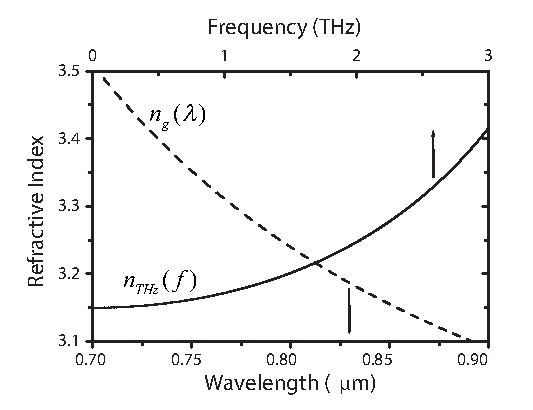
\includegraphics[width=0.65\linewidth]{Chapters/Experimental/Ref_index_ZnTe.pdf}
\caption{Group refractive index $n_g$ and phase refractive index $n_{THz}$ at optical and terahertz regimes, respectively, of ZnTe. Taken from \cite{PrinciplesofTHz}}
\label{fig:Ref_index_ZnTe}
\end{figure}



Finally, one has to consider the crystal's absorption in the spectral region of interest. The dominant causes of absorption in such crystals are the transverse-optical phonon resonances in the terahertz region. Table \ref{tab:THz phonons} lists such resonances in commonly used crystals.
\begin{table}[h!]
\caption{Lowest TO-phonon resonances in some EO crystals, taken from \cite{PrinciplesofTHz}}
\centering
\begin{tabular} {l c c c c c}
\hline
 & ZnTe & GaP & InP &GaAs&LiNbO$_{3}$  \\
\hline
$f_{TO}$ (THz) & 5.3 & 11 & 9.2 & 8.1 & 7.7 \\
\hline
\end{tabular}
\label{tab:THz phonons}
\end{table}





%%%---------%---%---------%---%---------%%%
%--------------THz Detection--------------%
%%%---------%---%---------%---%---------%%%
\subsubsection{THz Detection, Electro-Optic sampling} \label{sec:THz_det}
The THz detection mechanism used in this thesis is called Electro-Optic (EO) sampling. It falls out of eq. \eqref{eq:Pnl and chi} when we take the limit of $\omega_2 \to 0$,
\begin{equation}
P^{(2)}_i(\omega_1)=\epsilon_0 \sum_{j,k}\chi_{i,j,k}^{(2)}(\omega_1) E_j(\omega_1)E_k^{*}(0).
\label{eq:Pnl w1}
\end{equation}
From eq. \eqref{eq:Pnl w1} one can see that a DC electric field, $E_k^{*}(0)$, gives rise to a polarization $P^{(2)}_i(\omega_1)$ at frequency $\omega_1$. In other words, a static electric field induces a birefringence in the non-linear crystal proportional to the bias field amplitude. This effect is known as the Pockels effect. 

The detection of THz relies on the above process. The THz field strength is determined by the measuring the induced birefringence. This is achieved with polarization measurements of an optical probe pulse. Because the THz and visible light pulses have different temporal lengths (Fig. \ref{fig:THz_pulse}), the THz field is akin to a DC field when both pulses propagate through the EO crystal. Note, this only holds provided the THz wave and optical pulse travel at the same speed through the medium. The visible light pulse is scanned in time, via an optical delay line, to sample the full temporal THz waveform.



The electro-optic effect is weak. To enhance signal people use a balanced photo-diode detection scheme and a quarter wave-plate, shown in fig. \ref{fig:EO_sampling}. The quarter wave-plate is set to circularly polarize the probe beam if there is no THz present. A polarization beam splitter then sends equals amounts of power onto the balanced photo-diodes. Reading the difference in outputs from the diodes will yield zero. However, if the THz is present, the difference in outputs will correspond to the THz field amplitude. To further enhance signal, an optical chopper modulates the generation beam\footnote{Can also be the excitation beam} at half the repetition rate of the main laser. One then uses a Lock-In amplifier to only record the modulated signal. This minimizes electrical noise in the circuitry and intensity fluctuations in the main laser.
\begin{figure}[h!]\centering
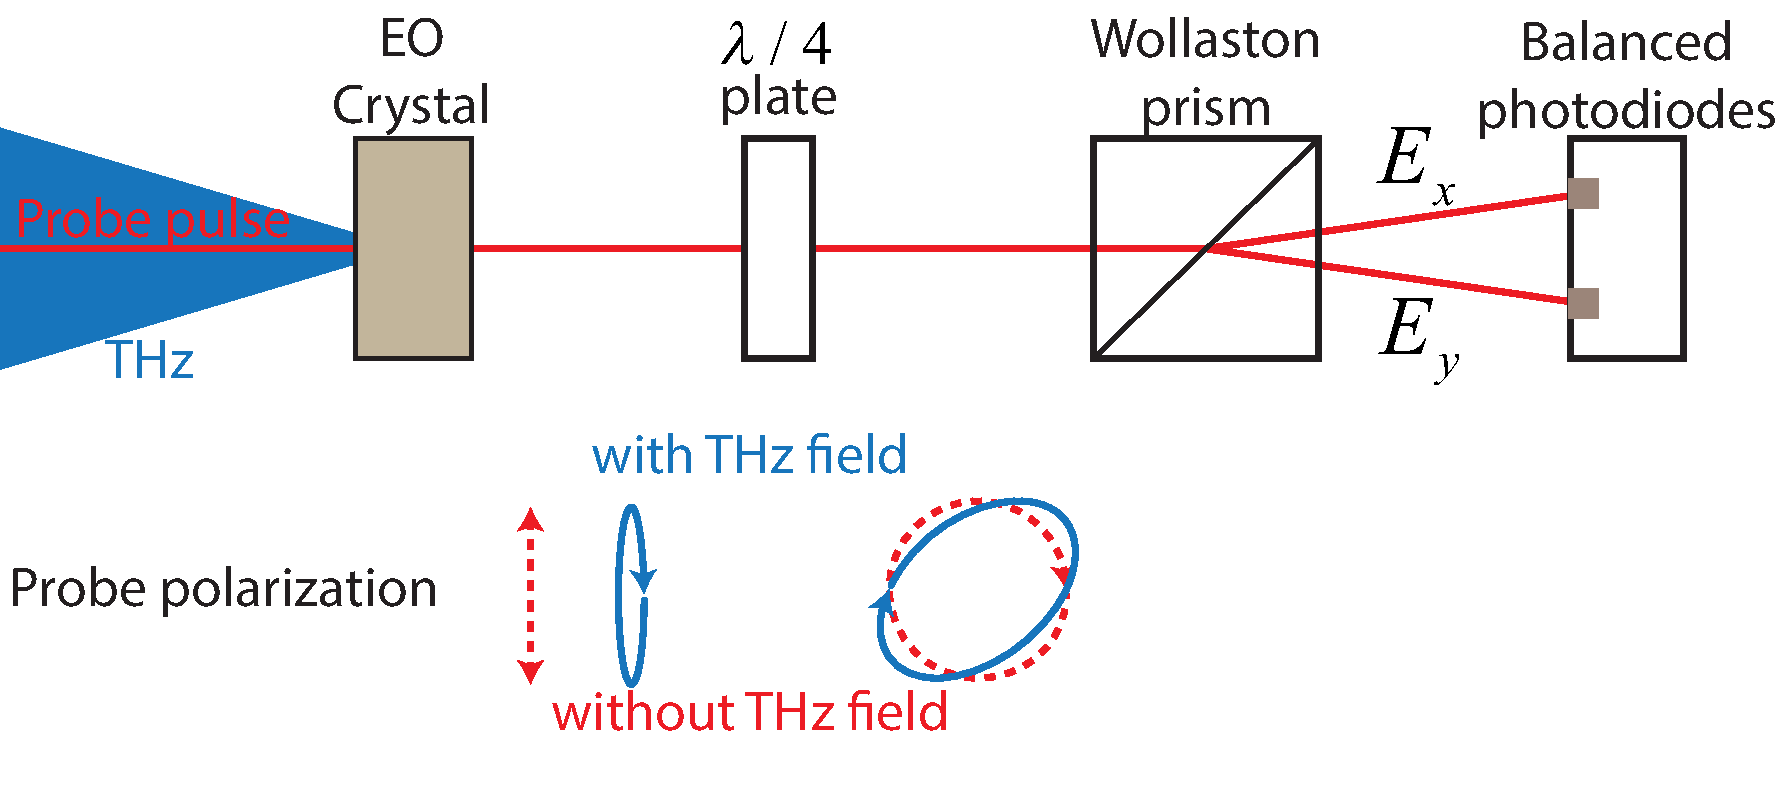
\includegraphics[width=0.73\linewidth]{Chapters/Experimental/EO_sampling.pdf}
\caption{A schematic of EO sampling. A focused THz pulse and a detection probe pulse are incident onto an EO crystal. Afterwards, the polarization of the probe pulse is measured by a pair of balanced photodiodes. A Wollaston prism is used to separate the orthogonal polarizations and a quater-wave plate is used to enhance the signal. Probe polarization with (solid) and without (dashed) the THz field are shown before and after the $\lambda /4$ plate.}
\label{fig:EO_sampling}
\end{figure}




%--------------------------------------------------%
%---%---%---%---%DIELECTRIC FUNCTION---%---%---%---%
%--------------------------------------------------%
\section{THz spectroscopic analysis}\label{sec:extract_perm}
Obtaining the frequency dependent refractive index of a sample is the standard use of a THz-TDS. Consider a pulse of radiation incident upon a slab of material. There will be a transmitted and a reflected pulse (see inset of fig. \ref{fig:extract_perm}\textbf{left}). The amplitudes of the transmitted and reflected pulses will be related to the incident pulse amplitude via the Fresnel reflection and transmission coefficients, \S\ref{sec:fresnel}. However, multiple reflections will occur within the material, as outlined in \S\ref{sec:Fabry_Perot}, hence the transmission and reflection functions of the material are respectively given by eqs. \eqref{eq:Fabry-Perot T} and \eqref{eq:Fabry-Perot R}. Therefore, if one has knowledge the incident wave and measures the transmission through (or reflection of) some material of known thickness, then it is possible to solve eq. \eqref{eq:Fabry-Perot T} for the refractive index of the material. We next outline how to extract the refractive index of a plastic cover slip with our system.

In our THz-TDS we perform two measurements: one measuring the temporal waveform transmitted through a sample, $E_{\mbox{samp}}(t)$, and the other to obtain a reference waveform without the sample , $E_{\mbox{ref}}(t)$. These two measurements are shown on the left of fig. \ref{fig:extract_perm}. Here one can see that the sample pulse (in red) is at a later time than the reference pulse (in blue). This is because it has traveled through the sample which has a larger refractive index than air\footnote{The reference pulse traveled through air.}. A small pulse at $\sim 14ps$ can be seen in the reference waveform, and it arises from the the first Fabry-Perot reflection in the material. Note, some fast oscillations can be see behind our main pulses. They were found to change depending on the optical alignment of our system, hence are associated with detector response function of our ZnTe crystal.

Our measurements contain the relative amplitudes and propagation times of our pulses, therefore a Fourier transform, eq. \eqref{eq:Fourier_T}, will yield the frequency spectrum and along with the relative phase of each frequency. The frequency spectrum and the phase of our THz pulses are shown on the right of fig. \ref{fig:extract_perm}. Here the solid blue and red lines show the detected transmission spectrum through free-space and our sample respectively. It can be seen that these two solid curves have the similar shapes, however the red curve has small oscillations in it. These are due to the first Fabry-Perot pulse detected in the time-domain measurement. The blue and red dashed lines show the phase\footnote{The unwrapped angle, shown here, is typically shown since it does not have $2 \pi$ discontinuities hence it has more visual appeal.} of the free-space and our sample waveforms respectively. One can see that the red dashed line has larger values of phase. This is because the sample waveform has accumulated a bigger phase delay by propagating through the sample. 
\begin{figure}[h!]\centering
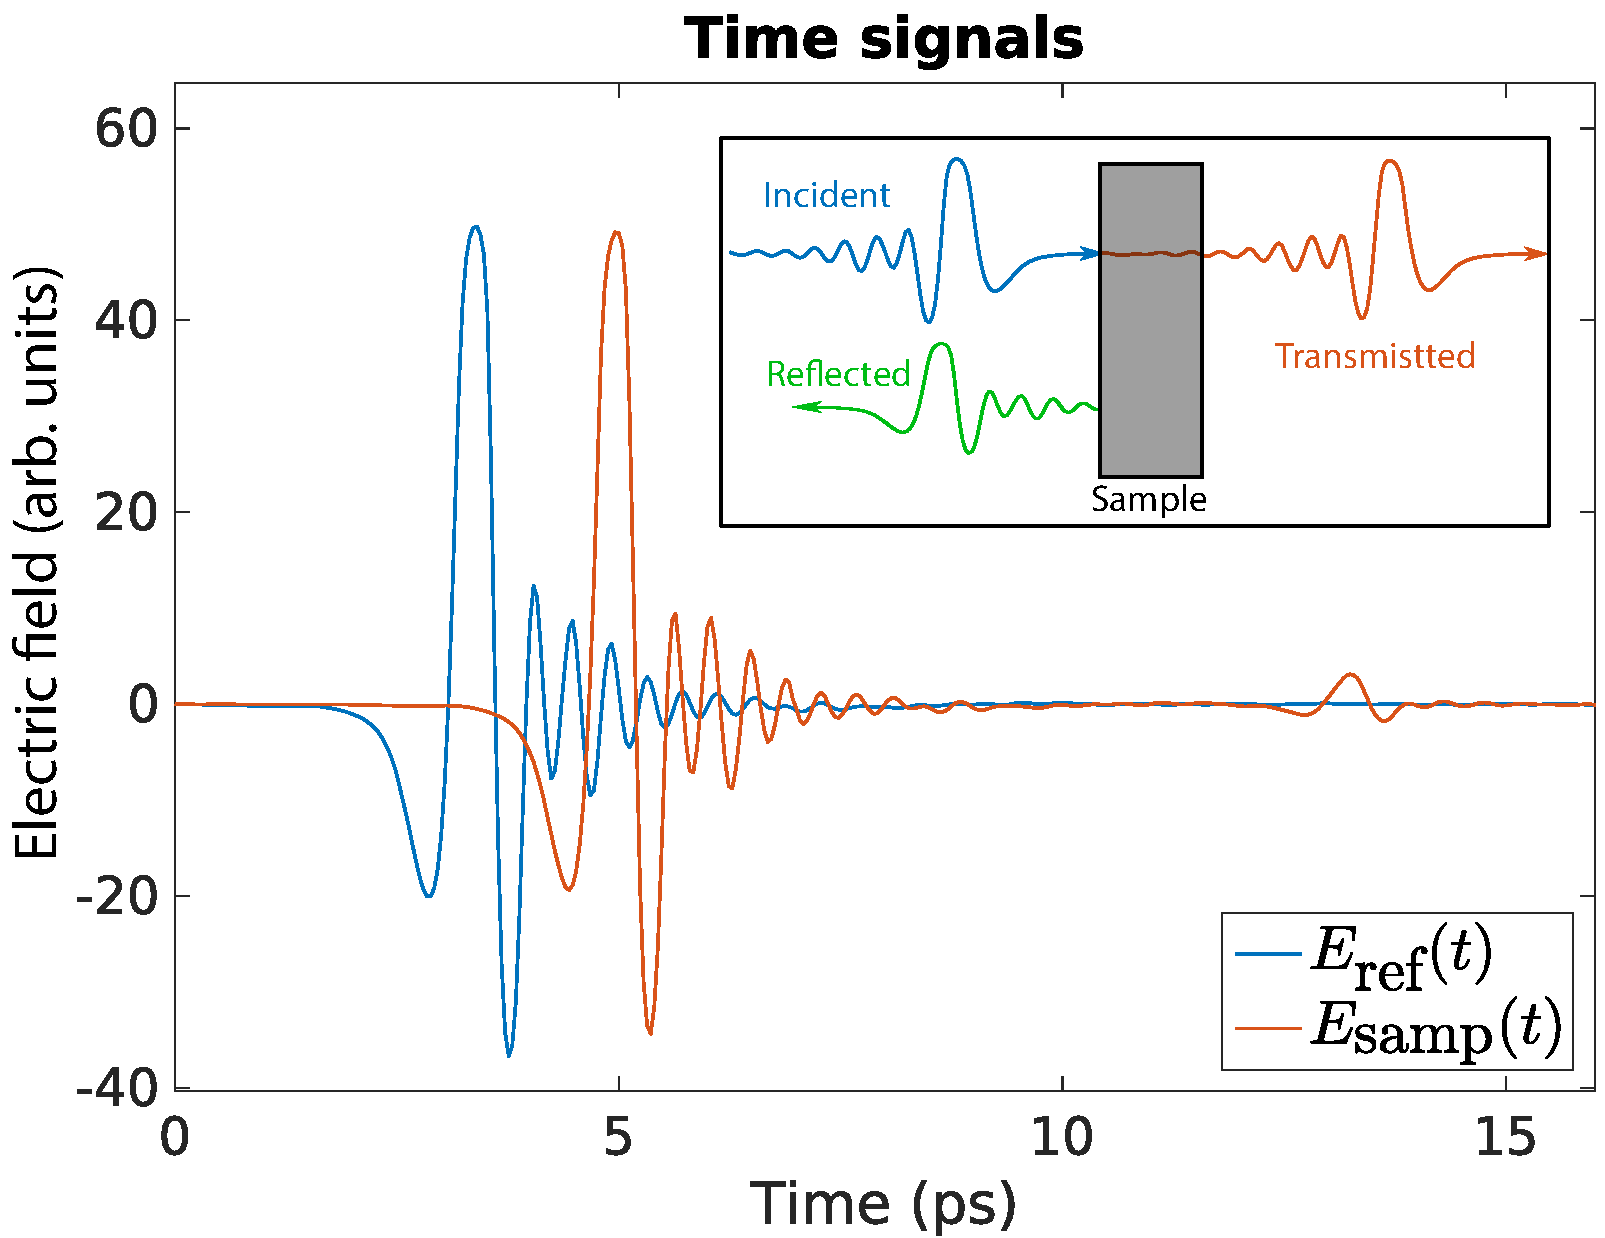
\includegraphics[width=0.465\linewidth]{Chapters/Experimental/time_data.pdf} %Updated this to say field strength
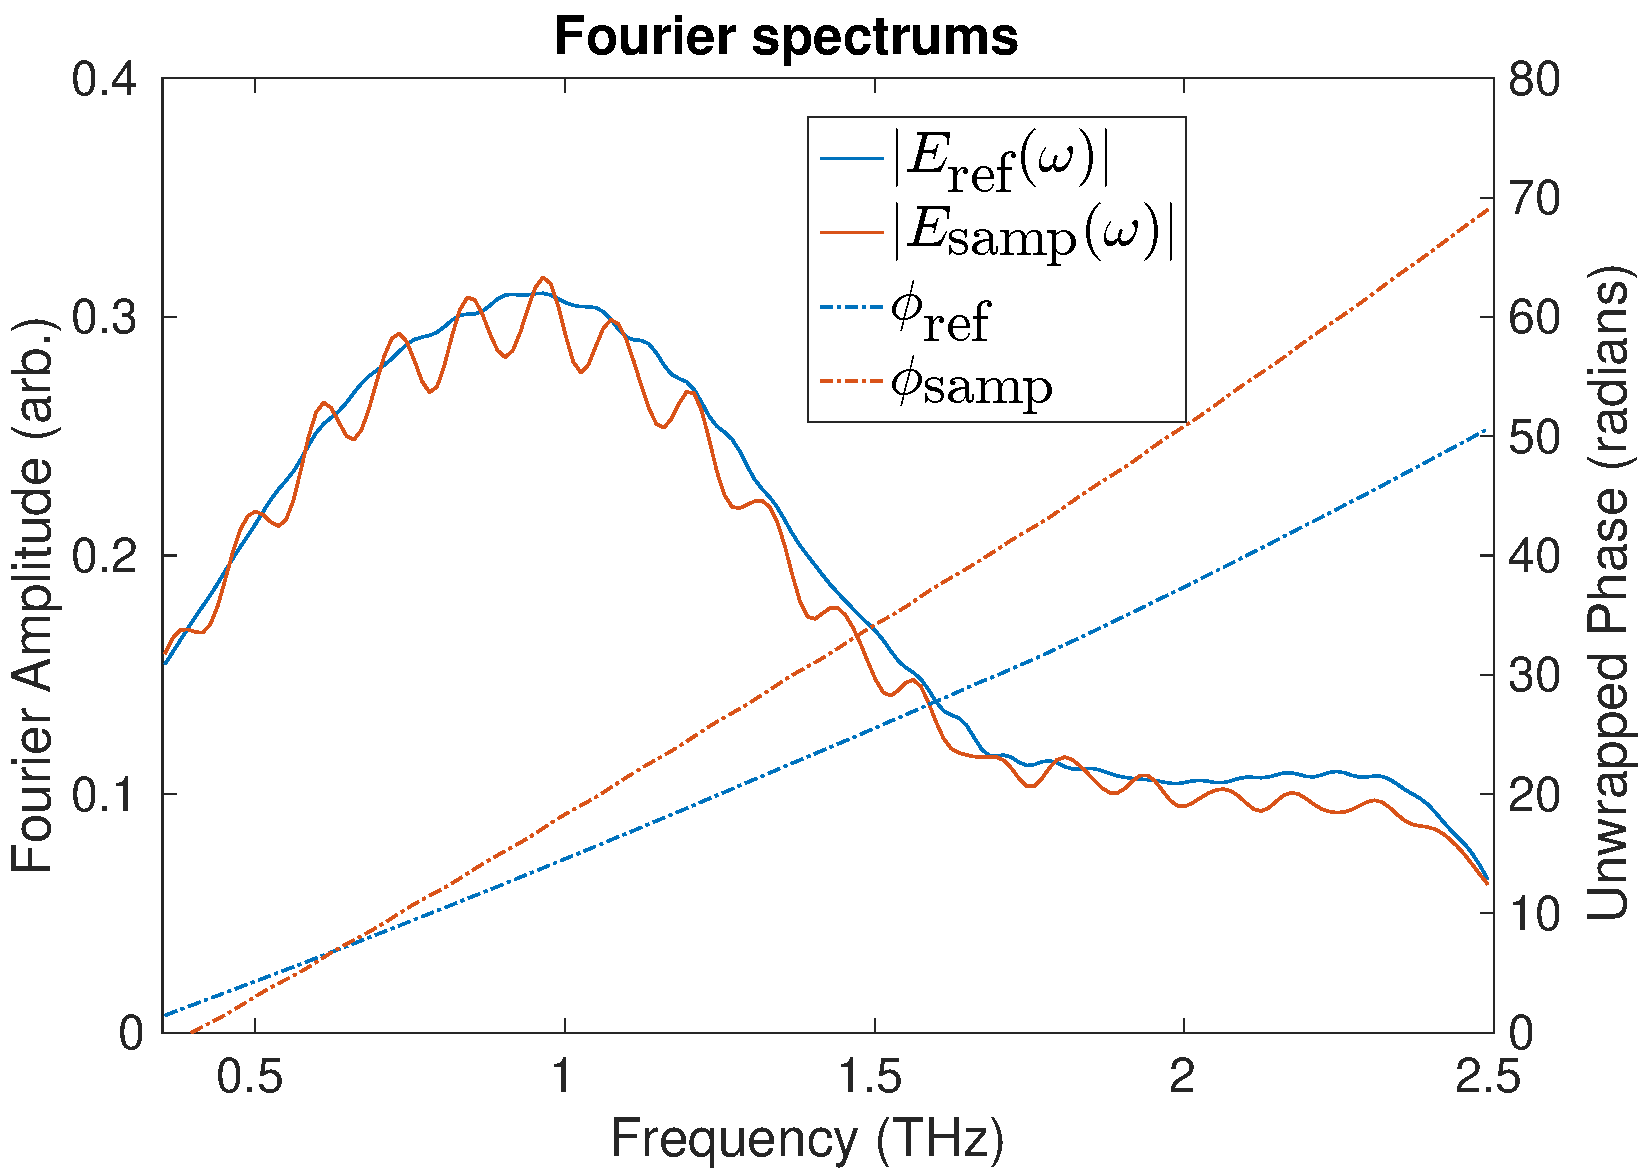
\includegraphics[width=0.505\linewidth]{Chapters/Experimental/Fourier_data.pdf}
\caption{\textbf{Left:} THz pulses measured by our system. Blue shows the reference pulse and the red trace shows the THz pulse transmitted through our plastic cover slip (this was a 810$\mu m$ thick plastic petry dish made from non-cytotoxic virgin polystyreneSterilin BS EN ISO 24998:2008). Inset shows a schematic illustration of the measurement. \textbf{Right:} Fourier spectrum of the THz pulses on the left. The solid lines are the power spectrum and dashed lines are the unwrapped phase where the blue (red) colour shows the data from the reference (sample) scan.} %Updated the caption to say details about plasic cover slip.
\label{fig:extract_perm}
\end{figure}

After the Fourier transformation, we have $E_{\mbox{ref}}(\omega)$ and $E_{\mbox{samp}}(\omega)$ which be substituted in eq. \eqref{eq:Fabry-Perot T}. Note, our reference measurement is related to the incident waveform by $E_{\mbox{ref}}(\omega) e^{-i\omega L/c}=E_i$, where $L$ is the sample thickness, since it has propagated through air with a refractive index of $1$. Therefore we obtain
\begin{equation}
\frac{E_{\mbox{samp}} (\omega) }{ E_{\mbox{ref}} (\omega) e^{-i\omega L/c}} = \frac{ t_1 t_2e^{i\phi_n} }{ 1 - r_1 r_2 e^{2i\phi_n} },
\label{eq:extract_perm}
\end{equation}
where $\phi_n = \omega n L /c$ is the phase delay the wave accumulates by propagating through our sample, $t_{1,2}, r_{1,2}$ are the relevant Fresnel coefficients, eqs. (\ref{eq:Fresnel para}-\ref{eq:Fresnel perp}). The only unknown left is the refractive index of our sample, $n$, which can be solved for numerically at each frequency point. Since our measurement contains the relative amplitudes and the relative phases, our solution can obtain the complex refractive index. However, since the phase term is $2 \pi$ periodic there is an infinite number of solutions that satisfy eq. \eqref{eq:extract_perm}. Therefore, selecting the correct solution is of vital importance. This accomplished by making an initial guess at the refractive index. This guess can be made by looking at the time difference between the reference and sample waveforms. If we denote the temporal co-ordinates of the peaks of the sample and reference waveforms as $t_s$ and $t_r$ respectively, one obtains
\begin{equation}
n_r = 1 + \frac{(t_s-t_r)c}{L}
\label{eq:int_real}
\end{equation}
as the real part of the average refractive index. For non-absorbing samples this will suffice. However, should the sample be absorbing then one can use the above value and 
\begin{equation}
\frac{|E_{\mbox{samp}}(\omega_c)|}{|E_{\mbox{ref}}(\omega_c)|} = t_1 t_2 e^{-n_{i} \omega_c L/c},
\label{eq:int_imag}
\end{equation}
where $\omega_c$ is the central angular frequency of the pulses and $n_{i}$ is the imaginary part of the refractive index, to obtain an initial guess for the imaginary part\footnote{This equation is only valid if we consider only the first transmitted pulse through our sample, ie. zero out the Fabry-Perot pulses in the temporal measurement}. A more accurate estimate is obtained by saying $t_{1,2}$ are also functions of $n_{i}$, however a numerical solver needs to then be used. Although crude, this initial guess will ensure that the numerical solver\footnote{The numerical solve we use is the \textit{vpasolve} function built into MATLAB 2016b.} of eq. \eqref{eq:extract_perm} will find the physically relevant solution. A technical note, this crude initial guess is used only for the first frequency point inputed into the solver. Then the solution from the first frequency point is used as the initial guess for the second frequency point.  This process is iterated until one has a solution for all the frequencies in the spectrum. This iterative process ensures that the obtained refractive index is a continuous function. 

\begin{figure}[h!]\centering
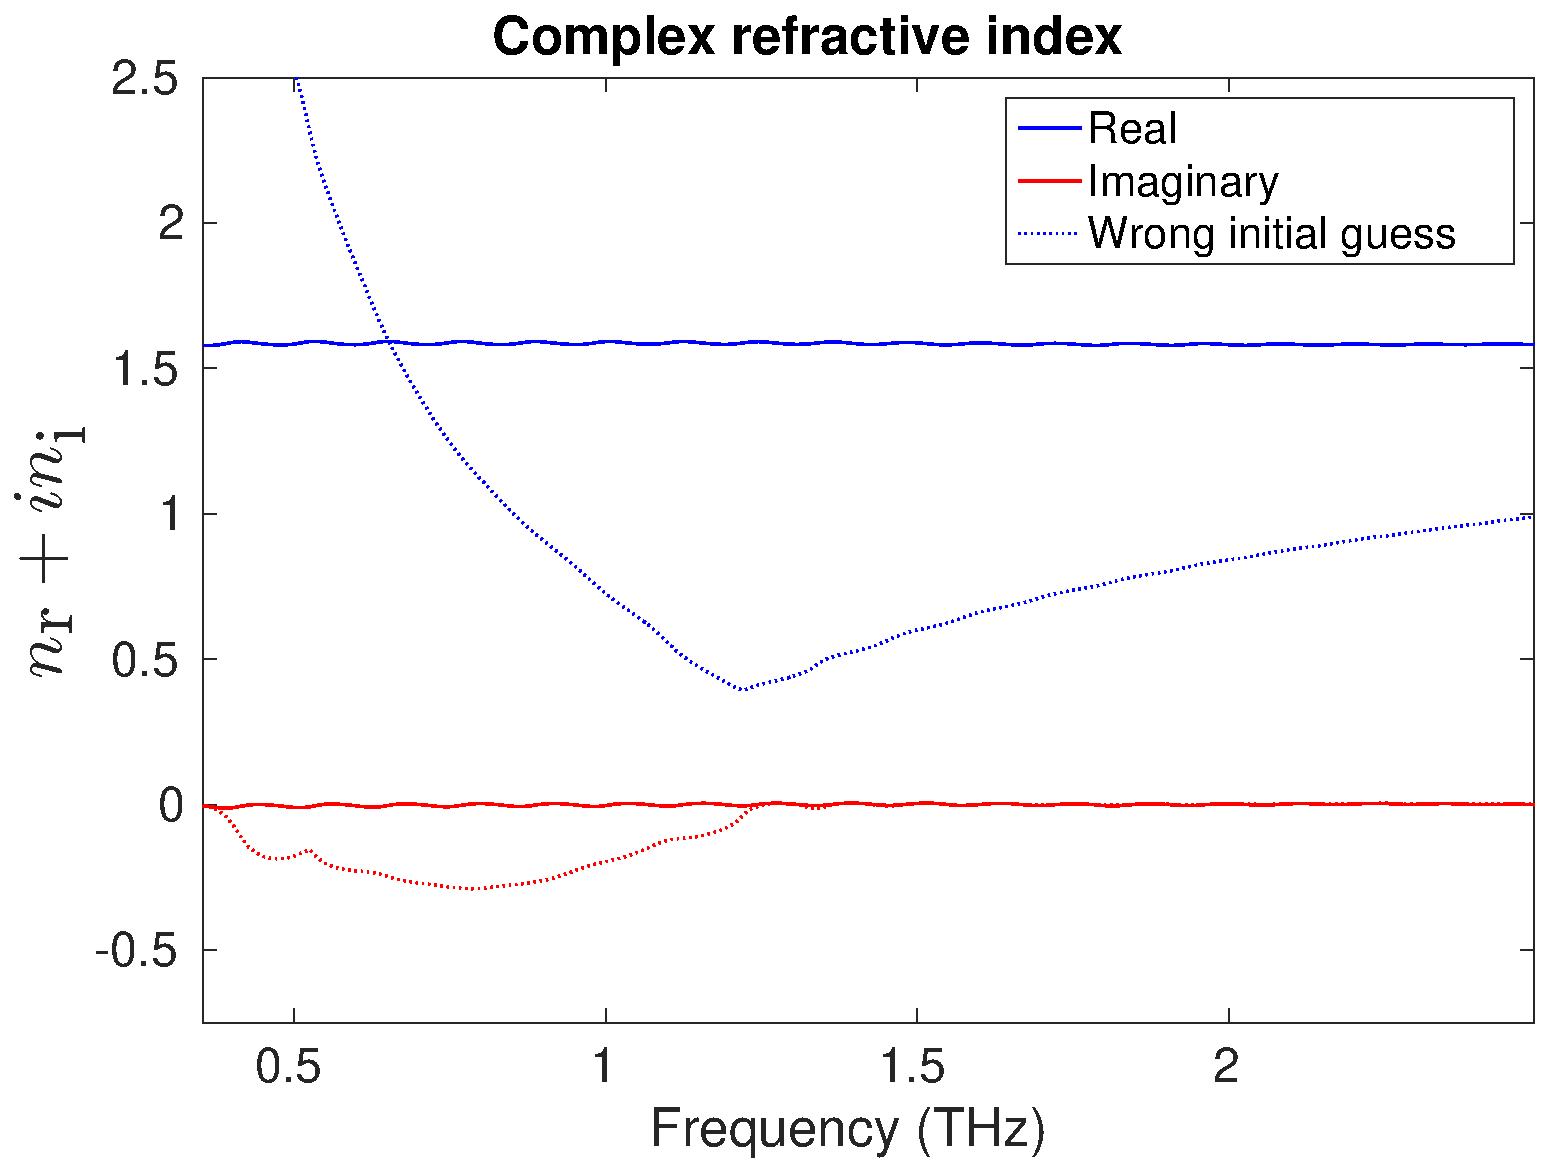
\includegraphics[width=0.66\linewidth]{Chapters/Experimental/ref_index.pdf}
\caption{Refractive index of plastic cover slip. Solid blue and red lines respectively show the real and imaginary refractive index with an initial guess of $n=1.50$. The dashed lines show the obtained refractive index with an initial guess with $n=3$.}
\label{fig:ref_index}
\end{figure}

Figure \ref{fig:ref_index} shows the real and imaginary refractive index of the plastic cover slip\footnote{This was a 810$\mu m$ thick plastic petry dish made from non-cytotoxic virgin polystyrene Sterilin BS EN ISO 24998:2008} used as a sample in the temporal measurements of fig. \ref{fig:extract_perm}. The solid lines show the obtained solution using the initial guess of eq. \eqref{eq:int_real} with the real (imaginary) part in blue (red). One can see a very flat dispersionless response with no absorption. However, one can see small oscillations. These are due to the fact that we have solved for the Fabry-Perot equation whereas in the temporal measurement we measured only the first Fabry-Perot pulse. The dotted lines show the obtained solution with an initial guess of $n=3$. This solution is obviously false since it means that we have gain from $0.3$ to $1.25THz$ in the imaginary part (dotted red line) and the real part (dotted blue line) is less than 1 from $0.8$ to $2.4THz$. 


%Added the next paragraph to say why this plastic very useful
This dispersion-less non-absorbing response from this type of plastic is very useful for THz measurements. The reason is they are originally designed to be used as petri dishes, hence they are non-toxic to bacteria, optically transparent, thermally resistant, mechanically rigid and readily available. These qualities make them excellent alternatives to glass cover slips, as used in the visible regime, since glasses absorb THz radiation. The optical transparency can in principle allow a THz and an optical image to be taken simultaneously. More over, the main imaging technique in this thesis (described in the later sections of this chapter) uses visible light to switch the material response of silicon from dielectric to metal (\S \ref{sec:THz_mod}), which has allowed the placement of a near-field THz probe next to a biological sample as shown in ch. \ref{c:cartilage}. 


\subsection{Multi-layer systems} \label{sec:multi-layers}
The previous section is only applicable if there are 3 materials, in other words the sample is free standing in space. However, if our sample is enclosed by two cover slips, ie. it is a multi-layered system, then it is convenient to use the transfer matrix method \cite{Ulbricht2011CarrierSpectroscopy}. As before, our measurement contains the transmission coefficients, however our transmission function of the system is \cite{Ulbricht2011CarrierSpectroscopy, multi_layers}
\begin{equation}
t=\frac{2 \sqrt{\epsilon_i}}{M_{21} + \sqrt{\epsilon_i} M_{11} + \sqrt{\epsilon_{f}}(M_{22}+\sqrt{\epsilon_i} M_{12})},
\label{eq:multi-layers}
\end{equation}
where $\epsilon_i$ and $\epsilon_{f}$ are the permittivities of the initial and final media, respectively, enclosing the multilayer system and $M$ is a $2\times2$ matrix associated with the propagation through the entire multilayer system. This matrix is given by the product of the individual layer matrices, $M\equiv M_1M_2M_3...M_N$, describing the propagation through each layer. The characteristic matrix of the $j^{\text{th}}$ layer, $M_j$, with thickness $l_j$ and dielectric function $\epsilon_j$ is given by
\begin{equation}
M_j = \left[ \begin{array}{cc} \cos\beta_j & \frac{-i}{\sqrt{\epsilon_j}}\sin\beta_j \\ -i\sqrt{\epsilon_j}\sin\beta_j & \cos\beta_j \end{array}\right],
\end{equation}
where $\beta_j=\omega l_j \sqrt{\epsilon_j}/c$ is the phase delay associated with light propagation inside the $j^{\text{th}}$ layer. By equating the experimental amplitude transmission coefficients $E_{\mbox{samp}}/E_{\mbox{ref}}$ with \eqref{eq:multi-layers}, we can then numerically solve for the permittivity of the sample as before. Then one can divide the transmission functions of the different systems and equate them to the experimental amplitudes. Note, it is of preference that the materials used in the reference measurement are not absorptive hence improve signal to noise.  

This multi-layer analysis allows one model much more complex systems than a simple Fabry-Perot model. We use this multi-layer analysis in chapter \ref{c:cartilage}.



%-----------------------------------------------------------%
%-----------------SILLICON PHOTOEXCITE----------------------%
%-----------------------------------------------------------%
\section{THz modulation via photoexcitation of Si} \label{sec:THz_mod}

\subsection{Silicon photoexcitation}

Undoped high-resist silicon is a dielectric for THz frequencies. It has a dispersion-less refractive index of 3.42 from $0.5 \mbox{ to } 4.5THz$ with minimal absorption \cite{THzsilicon}. It has very few charge carriers, therefore its Drude plasma frequency lies below the terahertz regime. However, if the number of charge carriers is increased via photoexcitation, then silicon can behave as a classical Drude conductor \cite{Photo.Si}. This has allowed for amplitude, phase and frequency modulation of THz via the optical excitation of silicon \cite{Photo.Si}. More recently, people have built upon these ideas to create an optically modulated wire-grid polarizer \cite{Siopticalpolarizer} in Silicon. There are other materials which have similar properties such as InSb and GaAs.


We next consider controlling the carrier density via optical excitation in our system. Consider the Drude model permittivity, \S\ref{sec:Drude Model},
\begin{equation}
\epsilon(\omega)=\epsilon_{\infty}+\frac{i \omega_p^2}{\omega(1/\tau-i\omega)}=\epsilon_{\infty}+\frac{i N e^2}{\epsilon_0 m \omega(1/\tau-i\omega)},
\label{eq:drude_perm}
\end{equation}
where $N$ is the number of charge carriers, $e$ is the electron charge and $\tau$ is the average carrier collision time (160$fs$ for undoped silicon \cite{Silicon_conduction}). Here, the number of charge carriers, the primary modulating parameter, is modulated via optical excitation with photons of energy $\hbar \omega$. When such pulses hit this material electrons in the valance band are given enough energy for them to enter the conduction band\footnote{This is provided the photons have enough energy to overcome the silicon bandgap of 1.12$eV$ (1100$nm$) at room temperature.}. In other words, they are no longer bound in the potential of the positive ion core they were orbiting and hence are able to traverse through the medium. Note, now there will also exist a vacant electron orbital referred to as a hole. Holes can travel through medium and act as though they have positive charge, thus are also considered as charge carriers. The excited electrons will then decay back down to their ground state and recombine with the vacant holes. The electron and hole populations at time $t$ after photoexcitation are given by $N(t)=N(0)e^{-\tau_c t}$, where $\tau_c$ is known as the carrier lifetime. In silicon the carrier lifetime is $25\mu s$ \cite{si_lifetime}. The repetition period of our pulses is 1$ms$, hence by the time our next pulse arrives all the carriers will have relaxed to their ground state. This allows us to neglect sample heating. Furthermore, since our THz-TDS allows us to probe our silicon picoseconds after photoexcitation, discussed in \S\ref{sec:photo_studies}, we can also neglect carrier recombination effects. The key variable to determine is therefore the mean carrier-carrier distance. In our system, we probe our material $5ps$ after photoexcitation, see Fig. \ref{fig:silicon_pump}, thus we can calculate the mean square displacement of carriers via eq. \eqref{eq:diffusion}. %$<x^2>=6Dt$ where $D$ is the diffusion coefficient of our electron (hole) charge carriers. Using the Einstein–Smoluchowski relation, eq. \ref{}, 
We obtain mean displacements of $\sqrt{<x^2>}=506nm(425nm)$\footnote{These numbers determine subsequent smearing and broadening of spatial features should an optical pattern be transferred to a THz beam using a silicon photomodulator. How we transfer an optical pattern to a THz beam is discussed in \S\ref{sec:optical_to_THz}.} for our photo-electrons (holes). Since the diffusion lengths are considerably smaller than the penetration depth of the photoexcitation light (12µm \cite{si_depth}), we can neglect carrier diffusion from our considerations. Therefore, one only needs to consider the carrier generation rate. We arrive at a charge carrier density of
\begin{equation}
N=\frac{I_0(1-R)}{2\hbar\omega A d}
\label{eq:Si carrier density}
\end{equation}
where $I_0$ is the incident intensity, $R$ is the reflectivity of Si at the incident wavelength, $d$ is the penetration depth and $A$ is the area of excitation. 


In all experiments involving silicon as the photomodulator, ch. \ref{c:1D_slit}, \ref{c:mod_thick}, \ref{c:noise_stability}, \ref{c:cartilage}, our pulse energy per unit area is $\sim 100\mu\text{J/cm}^2$, $R=0.3$ is the Fresnel reflectance of a Si interface at our excitation wavelengths, $\hbar \omega_l$ is the photon energy of the 800$nm$ pump light, $d$ is the penetration depth ($d$$\approx$$12\mu\text{m}$  \cite{si_depth} for our wavelengths) and the factor of 2 accounts for the excitation of electrons and holes. Using the average of the electron and hole masses, we obtain a Drude plasma frequency (eq. \ref{eq:plasma frequency}) of 70$THz$ with $\epsilon(1THz)=-101+36i$ for our photoexcited silicon. In other words, we generate a THz material with a negative real and positive imaginary part to the dielectric function, the characteristics of a lossy conductor.



\subsection{Photoexcitation studies with THz-TDS}\label{sec:photo_studies}
THz pump-probe spectroscopy allows one to study carrier photoexcitation and relaxation dynamics on picosecond time scales. This is achieved by investigating how the THz pulse changes at different excitation times. For now  we ignore what happens at different excitation times and return to this later. In figure \ref{fig:silicon_photo} we plot the THz pulses transmitted through undoped (solid line, $E_{\mbox{ref}}$) and photoexcited (dashed line, $E_{\mbox{photo}}$) silicon. For the undoped silicon, we can see the main THz pulse at $\sim 2ps$, then we see the 2$^{\mbox{nd}}$ and 3$^{\mbox{rd}}$ Fabry-Perot pulses arriving at $\sim 5ps$ and $\sim 7.5ps$ respectively. In the Fourier spectrum these secondary pulses manifest themselves as the Fabry-Perot peaks seen here. The pulse transmitted through the photoexcited silicon (dashed red line) is seen to have a similar shape as the other one and it arrives at the same time. However, the amplitude has been decreased by $\sim 85 \%$. This is because, as discussed in the previous section, we have generated a lossy conductor which has absorbed our THz radiation. Consequently, Fourier spectrum of this pulse has much lower amplitudes. 
\begin{figure}[h!]\centering
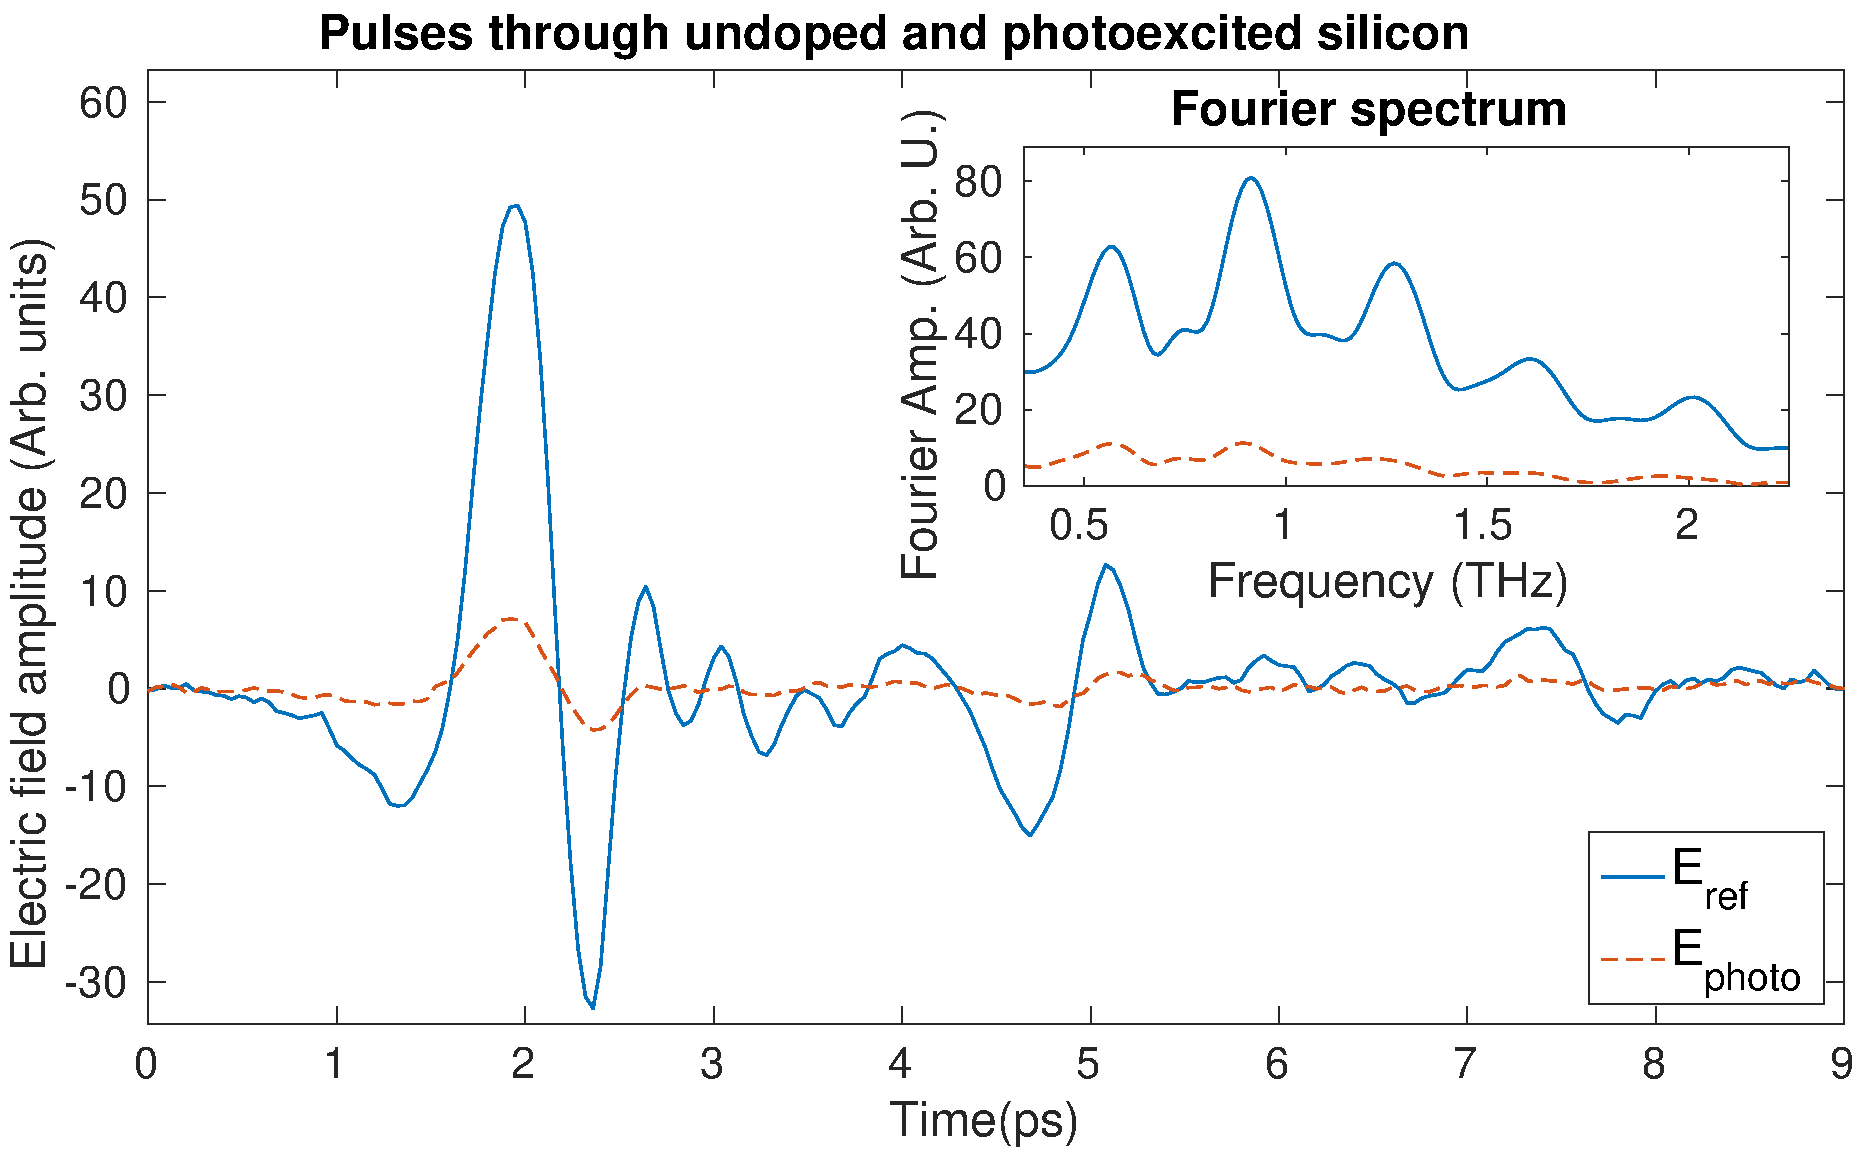
\includegraphics[width=0.80\linewidth]{Chapters/Experimental/silicon_photo.pdf}
\caption{THz pulses transmitted through an undoped (solid blue line) and a photoexcited (dashed red line) silicon wafer (115$\mu m$ thick, 1000$\Omega \cdot cm$ resist). Wafer is excited with 800$nm$ pump light with $\sim 100\mu J/cm^2$ fluence. Inset shows that Fourier transform of the pulses.}
\label{fig:silicon_photo}
\end{figure}

We can calculate the transmission of the photoexcited silicon from the the pulses in Fig. \ref{fig:silicon_photo}. This is achieved by dividing the spectra of the photoexcited pulse by the other one, ie. $|E_{\text{photo}} / E_{\text{ref}}|$.  This is what is plotted in figure \ref{fig:silicon_modulation} as the solid blue line. You can see that the transmission goes from 0.17 in our low frequencies to 0.07 in our higher frequencies.  From eq. \eqref{eq:drude_perm} the higher frequencies see a less absorbing material, however the shorter wavelengths see an optically thicker absorbing material. The latter mechanism seems to win over our frequency range hence the decrease in transmission. This is supported by modeling\footnote{Our model consists of calculating the transmission through a 2-layer system using eq. \eqref{eq:multi-layers}. The first layer is the photoexcited region of thickness 15$\mu m$ (a small amount more than the penetration depth) with permittivity given by eq. \eqref{eq:drude_perm} with $\omega_p=71THz$ and the second layer is undoped silicon of thickness 100$\mu m$ (wafer used in experiment was $115 \mu m$ thick).}. However, there is a mismatch in the number of peaks with experiment, namely there are 5 peaks in experiment and only 3 in modeling. This is because our model assumes a homogeneous photoexcitation layer where as in experiment the power is absorbed with an exponential decay rate with penetration depth of $12\mu m$. Thus in experiment there is no sharp boundary that the Fabry-Perot reflections to interact with. Note that due to the large silicon refractive index of $3.42$, the photoexcitation layer can not be assumed to be an infinitely thin sheet either. This mismatch changes the Fabry-Perot resonance conditions in experiment and modeling. Further, in experiment we have a small amount of water vapor present affecting our measurements.
\begin{figure}[h!]\centering
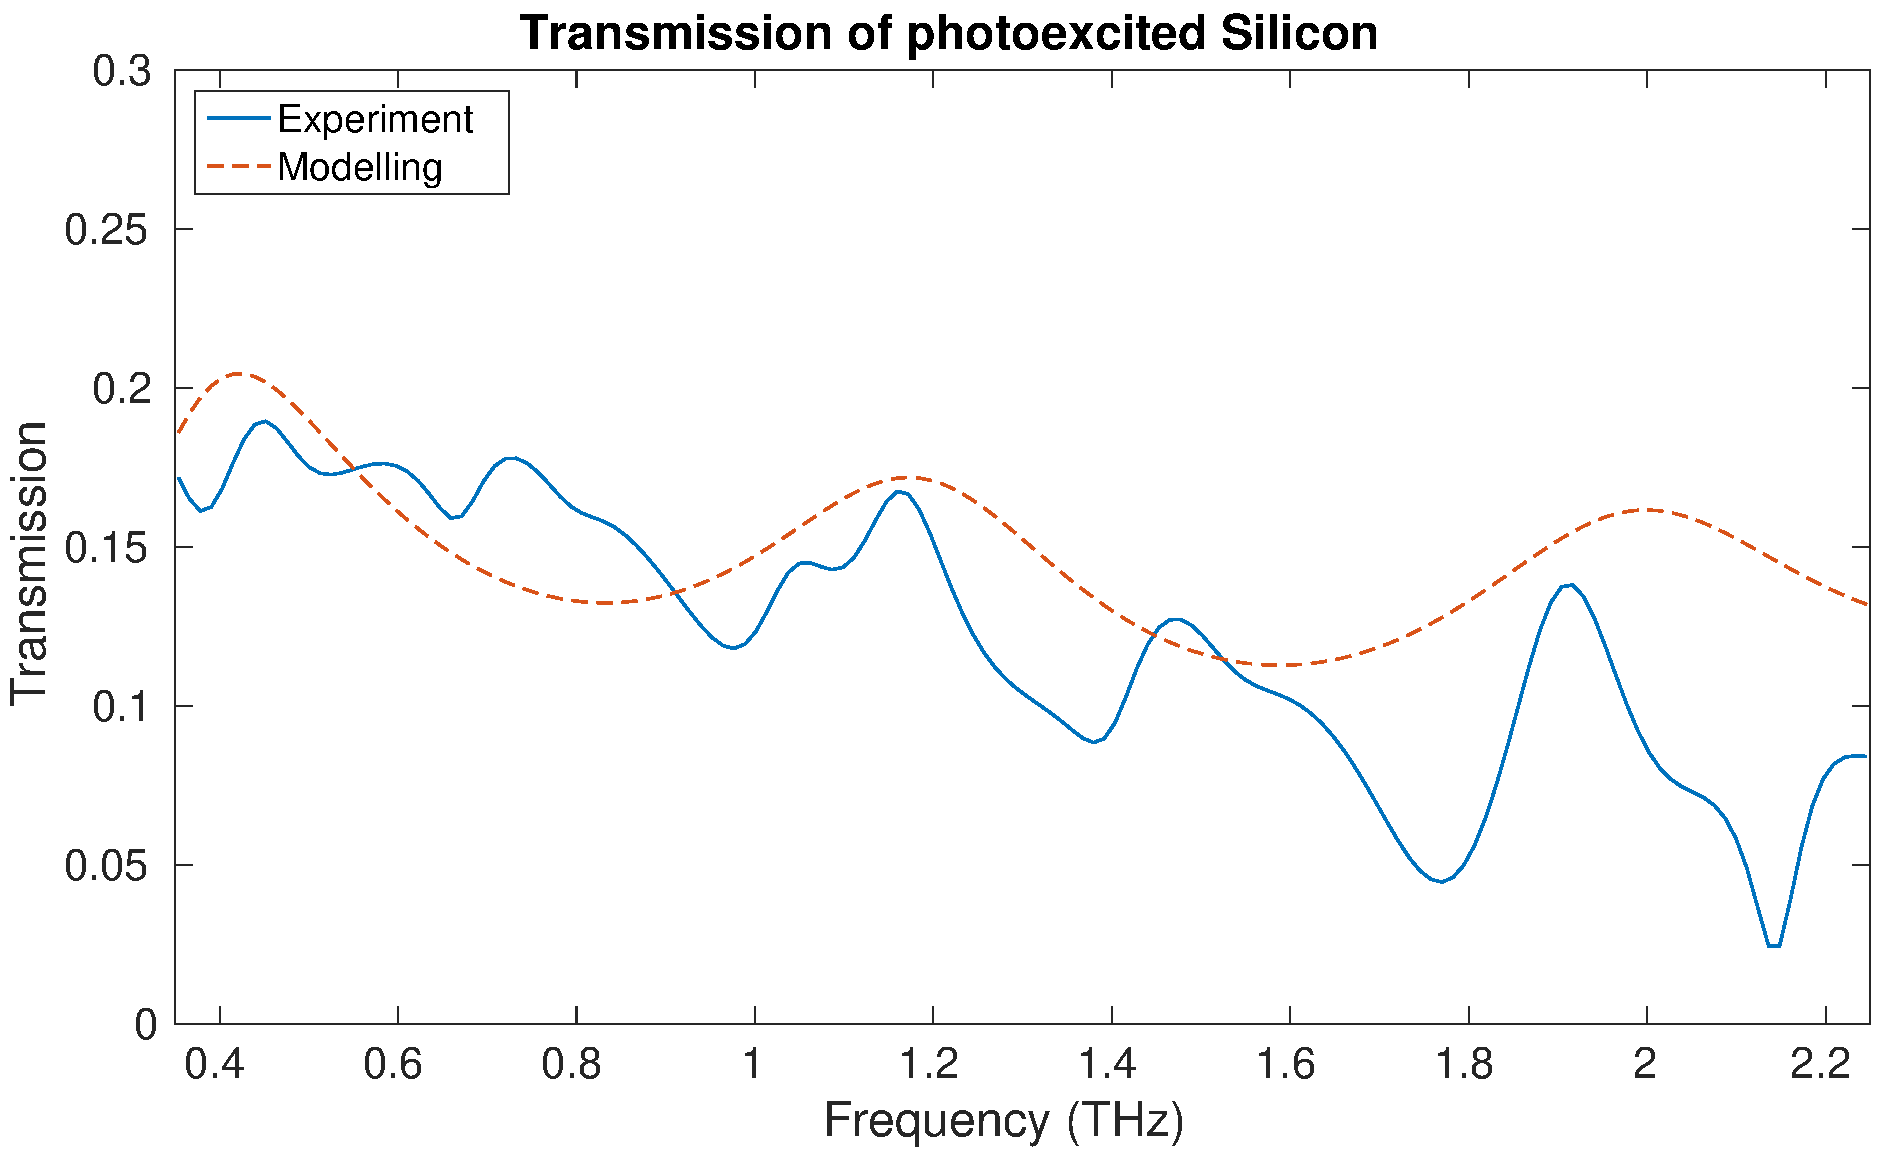
\includegraphics[width=0.80\linewidth]{Chapters/Experimental/silicon_modulation.pdf}
\caption{Amplitude transmission through photoexcited silicon with experiment and modeling in solid blue and dashed red lines respectively. There is a $\sim$2.5\% error in the experimental measurement. This error arises from the noise in the measurement of our THz waveforms, $\sim$5\% (see fig. \ref{fig:noise}), and the number of averages, 5, therefore rounding up the error is $\sim 5/\sqrt{5} \approx 2.5\%$.}
\label{fig:silicon_modulation}
\end{figure}

The previous two paragraphs have so far ignored what happens when we vary the arrival time of the pump excitation pulse. This is what will be considered next. For this we overlap our detection pulse overlapped with the peak of our THz waveform, as indicated in the inset of fig. \ref{fig:silicon_pump}. Then we change when our pump excitation pulse arrives at our silicon sample. Note, we measure the change in transmission due to photoexcitation, ie. $\Delta E = E_{\mbox{ref}} - E_{\mbox{photo}}$ from fig. \ref{fig:silicon_photo}. For negative arrival times the pump arrives after our THz pulse. Therefore, since the THz pulse has passed through the sample unphotoexcited, we do expect a value of zero for $\Delta E$. This is what we observe. When the pump pulse arrives at similar times as the THz pulse, we start to observe non-zero values. This is because the photoexcitation has started to generate charge carriers and thus change the permittivity. These photoexcited carriers will eventually relax back down to their ground state. However, in silicon carrier relaxation occurs on microsecond time scales \cite{si_lifetime} and our system measures up to a nanosecond difference in time delay\footnote{This is due to light traveling 30$cm$ in 1$ns$, hence the need for much longer delay lines.}. 
\begin{figure}[h!]\centering
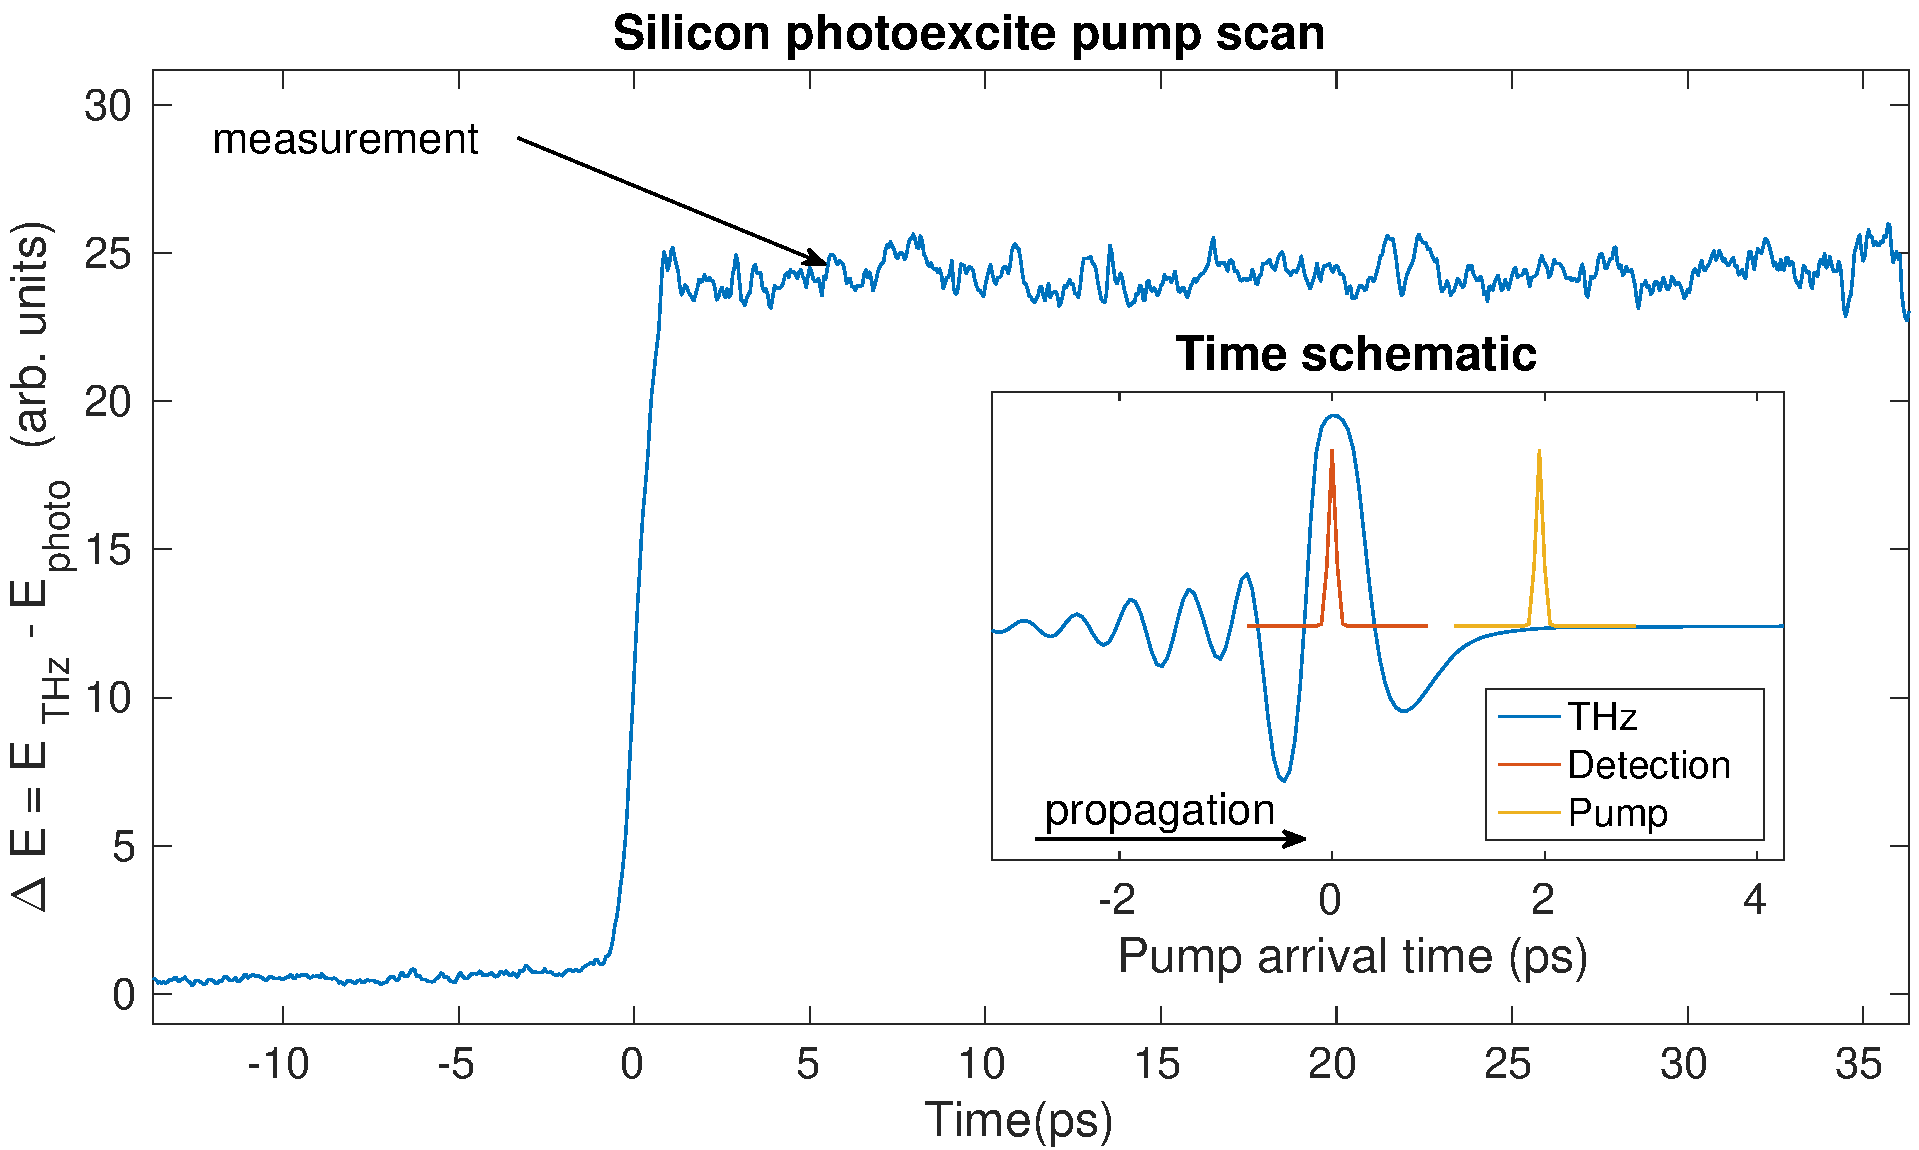
\includegraphics[width=0.80\linewidth]{Chapters/Experimental/silicon_pump.pdf} %Updated yaxis label and sorted the 5ps rize time.
\caption{Difference in THz transmission due to the photoexcitation of silicon. Inset shows a schematic illustrating when the pump pulse arrives on the sample with respect to the THz and detection pulses. Propagation arrow points the direction which the pulses are traveling.}
\label{fig:silicon_pump}
\end{figure}

The black arrow labeled as ``measurement'' indicates when the pump pulse arrives on our silicon wafer when we use the photoexcitation of silicon for imaging with a single-element detector, discussed in the next section.






%-----------------------------------------------------------%
%-----------------Single pixel imaging----------------------%
%-----------------------------------------------------------%
\section{Imaging with a Single-Element Detector}\label{sec:single_pixel_imaging}
THz detector arrays are currently difficult and expensive to manufacture \cite{T-ray_sensing}. As a consequence, we can not use array based imaging techniques, such as those used in the modern day cameras, where one uses a lens to project an image of some scene on a detector array, thereby obtaining the intensity (or amplitude) of each spatial point of the scene simultaneously. Our detector can only measure the total amplitude emanating from the scene, hence why it is called a single-element detector. The simplest way of imaging with such a detector is to block the light from the entire scene leaving only a small square to be transmissive, an aperture. Then our detector readout will correspond to the light emanating from that small square, the first pixel in our image. If we move the aperture and measure again, then we will the know the light emanating from the area adjacent to our first measurement. This process is iterated until we have sampled the entire scene. In other words, our imaging measurements are obtained sequentially rather than in parallel. For this reason, single-element imaging typically has a longer acquisition time compared to focal plane imaging arrays, its major disadvantage. However, single-element detectors are generally cheaper and more robust.

The resolution of a raster scanning technique, as outlined above, is determined by size of the aperture. However, if this aperture is made smaller and smaller, the light reaching our detector is reduced and eventually one will run into detector noise. 

One could sample more than one aperture simultaneously to increase the detected signal level in order to overcome detector noise, an idea which seems to first originate in 1935 with Yates \cite{Yates}. This idea is illustrated in fig. \ref{fig:1px_imaging}. Here, we have a light source shining upon a spatial encoding mask (ie. it has many apertures open as opposed to one). This spatially encodes a beam of radiation, and then this beam passes through an object and all the light is gathered by a single-element detector. In the next measurement we change the configuration of our encoding mask (ie. change the location of the apertures) and measure again. Although we have increased the light reaching our detector in each measurement, to form an image with such encoding masks, however, introduces extra calculation difficulties as the measured intensity is due to the sum of the scanning apertures. Therefore, the mask configurations (the locations of the scanning apertures) in each measurement must form a set of simultaneous equations which can be solved for the individual pixels of the object’s transmission function.

\begin{figure}[h!]\centering
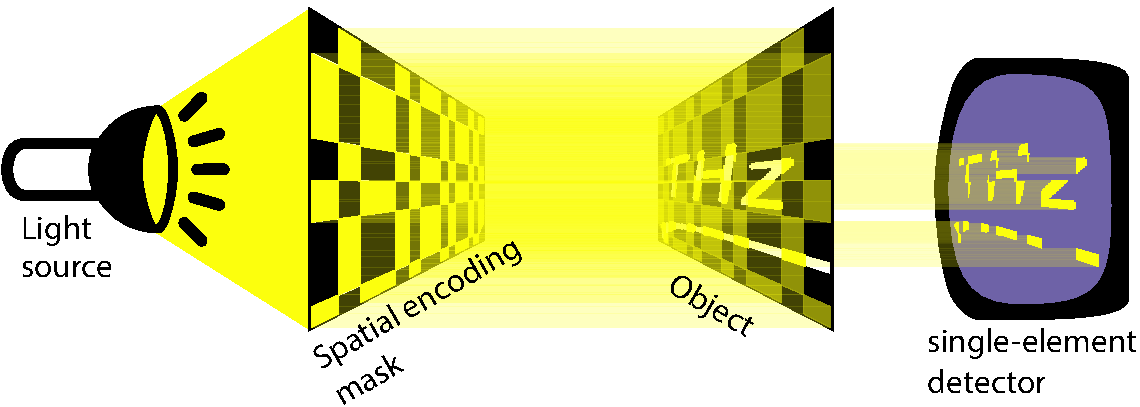
\includegraphics[width=0.90\linewidth]{Chapters/Experimental/1px_imaging.pdf}
\caption{Imaging with a single-element detector. An encoding mask spatially encodes a beam of radiation. Follow this, the beam is passed through an object and onto the single-element detector.}
\label{fig:1px_imaging}
\end{figure}



We now consider the construction of an $N$-pixel image $\mathbf{y}$; our $i^{\text{th}}$ measurement, $y_i$, is the dot product of the object transmission function and the $i^{\text{th}}$ mask configuration, mathematically expressed as 
\begin{equation}
y_i=\sum_{j=1}^N a_{ij}x_j,
\label{eq:phi_i}
\end{equation}
where $a_{ij}$ holds the spatial information of the $i^{\text{th}}$ mask and $x_j$ is the $j^{\text{th}}$ pixel of the object. The full set of measurements can be represented by the matrix equation 
\begin{equation}
\mathbf{y}=A\mathbf{x},
\label{eq:y=Ax}
\end{equation}
where the rows of matrix $A$ are shaped into the projected masks. For invertible matrices $A$, the image vector $\mathbf{x}$ can be obtained through matrix inversion $\mathbf{x}=A^{-1}\mathbf{y}$. Otherwise, one can use least squares solvers and more complicated recovery algorithms. Note that $\mathbf{x}$ then has to be reshaped into a 2D matrix of pixel values. A note on terminology, the matrix equation \eqref{eq:y=Ax} represents the image being expanded in some basis given by $A$ and they are discussed in \S\ref{ss:masking_scheme}. 


\subsection{Implementation in the THz regime}\label{sec:optical_to_THz}
\begin{figure}[b!]\centering
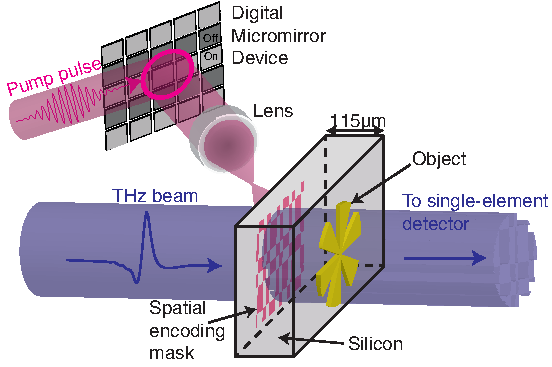
\includegraphics[width=0.68\linewidth]{Chapters/Experimental/THz_imager.pdf}
\caption{\textbf{Single pixel THz imaging}: An 800nm pump pulse is spatially modulated and used to photoexcite a semiconducting wafer, which transfers the spatial encoding mask onto a coincident THz pulse. The subsequent THz pulse is then passed through an object onto a single pixel detector.}
\label{fig:THz_imager}
\end{figure}
As discussed in \S\ref{sec:THz_mod}, the material response of an undoped Silicon wafer  can be switched from dielectric to conducting via photoexcitation with high energy pulses, ie. it can be made to absorb and block our THz radiation. Therefore, to spatially pattern our THz we can photoexcite this silicon wafer with the desired spatial pattern. To this end, we use a digital micromirror device\footnote{We use the DLP lightcrafter evaluation module by Texas instruments.} (DMD) to impart a spatial structure into the pump beam used to photoexcite the silicon wafer, as illustrated by Fig. \ref{fig:THz_imager}. The photoexcited regions have values of 0, in eq. \eqref{eq:y=Ax}, since they absorb our THz radiation where as the other regions transmit THz and thus they have values of 1. Then we pass our THz pulse through this spatially photoexcited space, then through an object and finally on our single-element detector.

%As mentioned in \S\ref{sec:THz_det}, we use a Lock-In detection scheme which blocks half of our THz pulses. We can however modulate our pump beam instead of modulating our THz beam. In particular, use the DMD to change the projected patterns in synchronization with the main laser. Further, if we tell the DMD to switch between only two patterns, then the Lock-In amplifier will tell us the difference between the two patterns. This means the second pattern, the subtracted one, will have values of -1. This allows for the use of masks with values of 1s, 0s and -1s. This is especially beneficial when using orthogonal masking patterns, see \S\ref{sec:had_mat}.


Our physical masks are composed of 1s and 0s whereas some encoding schemes might be made of +1s and -1s, for example orthogonal masks derived from Hadamard matrices. However, as is outlined in \cite{hadamard_multiplex}, we can still perform a measurement with masks made +1s and -1s in our system. Consider the $H_2$ matrix and two other matrices $G^+$ and $G^-$:
\begin{equation}
H_2=\left[{\begin{array}{cc}1 & 1 \\ 1 & -1 \end{array} }\right],
\; \; \; \; \;
G^+=\left[{\begin{array}{cc}1 & 1 \\ 1 & 0 \end{array} }\right],
\; \; \; \; \;
G^-=\left[{\begin{array}{cc}0 & 0 \\ 0 & 1 \end{array} }\right].
\label{eq:H2}
\end{equation}
It is easy to see that $H_2=G^+ - G^-$. Thus if we have two sets of measurement vectors each using one of the complementary sets of masks, $\mathbf{y}^+=G^+\mathbf{x} \; \text{and } \mathbf{y}^-=G^-\mathbf{x}$, then subtraction of the second set gives the desired encoding matrix. This doubles the number of measurements required. However, due to detection scheme used, discussed in \S \ref{sec:THz_det}, the difference in THz transmission is obtained via a Lock-In amplifier. Our DMD is triggered by the main laser to switch between the $+ve$ and $-ve$ masks. This prevents doubling the total measurement time. This is because we use a Lock-In to detect the difference when the THz is switched on and off onto our detector. Moreover, since the complementary negative mask is projected immediately after its positive counterpart, one can eliminate an unwanted source of noise, namely low frequency source oscillations as shown in \S\ref{sec:low_freq_source}. 

\newpage
\subsubsection{Phase Front Correction}\label{sec:DMD_phase}
%\begin{wrapfigure}{r}{0.47\linewidth}
\begin{figure}[h]\centering
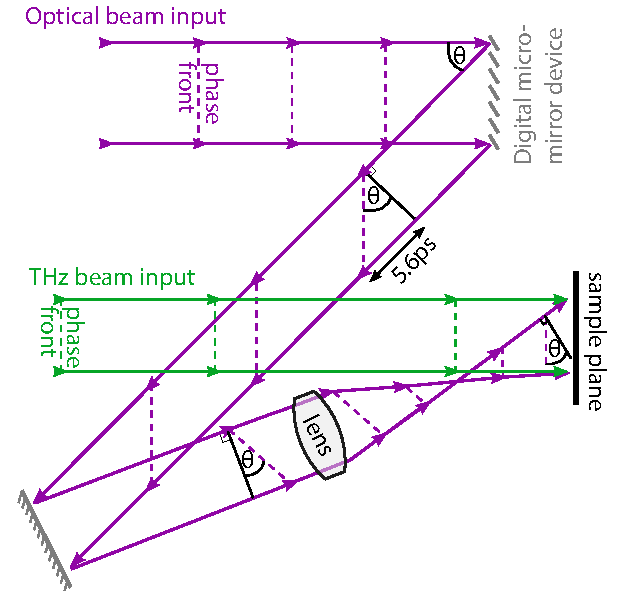
\includegraphics[width=0.65\linewidth, trim={1mm 2mm 1mm 0mm},clip]{Chapters/Experimental/temporal_smearing.pdf}
\caption{Diagram of the optical excitation scheme showing how a flat phase front is achieved with off axis photoexcitation. Each micro-mirror tilts at $\theta = 13^o$ to DMD array plane.}
\label{thzphase} 
%\end{wrapfigure}
\end{figure}
It needs to be mentioned that there is a phase front distortion induced by the DMD. This phase front distortion arises from the fact that each individual mirror tilts on its own at a 13$^{\circ}$ angle with respect to the overall mirror plane. This shortens, or lengthens, the optical path length of light hitting a mirror on the edge of the DMD array compared to one in the middle, as shown in fig. \ref{thzphase}. This means one will photo-excite different parts of the sample at different times. Therefore, if one wishes to study ultra-fast carrier dynamics, in graphene for example (see ch. \ref{c:graphene}), this wavefront distortion needs to be removed. This is achieved by photoexciting at an angle off normal opposite to the angle of the DMD mirrors. Figure \ref{thzphase} clarifies the arrangement used to achieve a photo-excitation without a temporally smeared wavefront.


\subsection{Choice of basis: Raster, Orthogonal, Random} \label{ss:masking_scheme}
Next we outline the ideas behind using three different measurement matrices, namely the identity matrix, orthogonal and random matrices. How each one of these performs in noisy experimental conditions is shown in chapter \ref{c:noise_stability}.

\subsubsection{Raster Scanning}
As pointed out earlier, we can raster scan a single aperture across our field of view. This means our $i^{\text{th}}$ measurement directly corresponds to $i^{\text{th}}$ pixel of our image. In the matrix notation of eq. \eqref{eq:y=Ax}, $A$ is the identity matrix $I_N$. 

There is one great disadvantage to using raster scanning techniques. Namely that to increase resolution the aperture size is reduced, however this also reduces the amount of light transmitted through an aperture. Therefore, by continual decrease of the aperture size eventually one will only measure detector noise. For apertures much larger than the wavelength the amplitude transmission is proportional to the area, i.e. $E \propto r^2$ where $r$ is the aperture radius and $E$ is the transmitted field amplitude. However, when the aperture size is smaller than the wavelength the dependence is described by Bethe's theory \cite{Bethe1944}, mathematically  $E \propto r^3$. This has already been demonstrated for THz frequencies \cite{THz_apertures} and such apertures can achieve $3\mu m$ spatial resolution \cite{Image.3um_probes}. It also possible to overcome the small transmissions of apertures and use near-field scattering tips \cite{Image.Near-Fields} in order to reach $nm$ resolution \cite{Image.STM,Image.Nanoscope1}. Whilst impressive, raster scanning techniques necessitate long measurement times due to the small signals emanating from sub-wavelength scatterers.



%Since the identity matrix consists of 1s and 0s, it does not have a $+ve$ and a complimentary $-ve$ mask. This prevents the use of a Lock-In amplifier to obtain the difference between complimentary mask pairs. Whilst this may seem as a disadvantage, the main benefit of such a measurement is the minimization of low frequency source oscillations (shown in the next section). However, since single apertures reduce the total transmission, they also reduce the effect of low frequency source oscillations. Therefore, raster scanning does not experience great losses from missing $+ve$ and $-ve$ mask pairs.

\subsubsection{Orthogonal Hadamard matrices} \label{sec:had_mat}
In this section, we use orthogonal Hadamard matrices as our basis expansion. So, $A$ is a Hadamard matrix of order $N$. A Hadamard matrix $H_n$ is defined as an $n\times n$ matrix of +1s and -1s with the property that the scalar product between any two distinct rows is 0 (each row is orthogonal to every other one). Thus $H_n$ satisfies:
\begin{equation}
H_nH_n^T=H_n^TH_n=nI_n,
\label{eq:H_n}
\end{equation}
where $H_n^T$ is the transpose of $H_n$. This allows for easy image reconstruction since $H_n^{-1}=H_n^T/n$, which is equivalent to summing the projected patterns with each pattern weighted by its detector readout. 

Every Hadamard mask (apart from the first one which is all 1s) has equal amounts of 1s and -1s, therefore in every measurement we use half of the total incident light. Therefore, a Hadamard basis will minimize the effect of detector noise \cite{H_optics}. This is the major reason why one should use a Hadamard sampling matrix. However, it should be noted that this Hadamard imaging scheme is quite sensitive to source noise. To explain this we modify eq. \eqref{eq:y=Ax} into $\mathbf{Ry}=A\mathbf{x}$ where $\mathbf{R}$ is an $N$-sized vector with the $i^{\text{th}}$ entry describing our source's power output at the time of measurement and $\mathbf{y}$ is the noiseless measurement vector. The $i^{\text{th}}$ entry of $\mathbf{R}$ is the total power transmitted through the $i^{\text{th}}$ mask, in other words the sum of the dot product between the $i^{\text{th}}$ mask and source power output at the time of measurement. With Hadamard masks we use of half of the total light in each measurement. Therefore, 5\% source noise fluctuations manifest themselves as 2.5\% noise fluctuations in $\mathbf{R}$.  For this reason, Hadamard imaging schemes are much more sensitive to source noise than raster scanning schemes\footnote{In raster scanning we only use very small amounts light in each measurement, hence source noise minimized}. Although source noise can be minimized by using $+ve$ and $-ve$ mask pairs, as demonstrated in \S\ref{sec:low_freq_source}, it still makes this Hadamard scheme unfavorable should one have a noisy source but a low-noise detector.

The most common method of constructing Hadamard matrices is via the \textit{Sylvester construction method}, first used in the 1860s. If we have some Hadamard matrix $H_n$ of order $n$, then 
\begin{equation}
H_{2n}=\left[{\begin{array}{cc}H_n & H_n \\ H_n & -H_n \end{array} }\right].
\label{eq:sylver_had}
\end{equation}
The lowest Hadamard matrix is $H_1=[1]$, therefore using eq. \eqref{eq:sylver_had} one can construct matrix of order $2^k$ where $k$ is a real integer. This is the most common method due to its simplicity, however it can be quite restrictive in terms of the number of pixels one can use, namely only powers of 2. Further more, for an $N \times N$ image one needs an $N^2 \times N^2$ matrix, which can cause memory problems when $N>512$. 

There is another construction method, the \textit{Paley construction technique}. Let $q$ be a prime power congruent to $3(\mod 4)$. Then one constructs a vector, $V$, of length $q$ in which the $i^{\mbox{th}}$ entry equals $\chi(i-1)$, where 
\begin{equation}
\chi (x) = \left\{ 
\begin{aligned}
0 \;& \mbox{ if } \;x=0\\
1 \;& \mbox{ if } \;x \mbox{ is a quadratic residue of }q\\
-1 \;& \mbox{ if } \;x\mbox{ is a quadratic non-residue of }q.
\end{aligned}
\right.
\label{eq:chi_quad}
\end{equation}
Then one constructs a $q \times q$ matrix, $Q$, where the $j^{\mbox{th}}$ row is obtained by cyclically permuting $V$ to the right $j-1$ times. Finally,
\begin{equation}
H_{q+1}= I + \left[{\begin{array}{cc}0 & J^T \\ -J & Q \end{array} }\right],
\label{eq:paley_had}
\end{equation}
where $J$ is a column vector of length $q$ where every entry equals $1$ and $I$ is the identity matrix. This method has two great advantages over the Sylvester method. First, it has greater freedom in terms of how many pixels one can sample since the allowed matrices are of order $q+1$ where $q$ is a prime congruent to $3 (\mod 4)$. Second, due to the cyclic permutation of $V$, one can construct each individual mask whilst only holding a vector of length $(N-1)^2$ in memory. 

Note, when creating masks of subwavelength dimensions, as in this thesis, then polarization effects in the masks need to be considered. This is done in \S\ref{sec:photo_gratings}. 


\subsubsection{Random matrices}
In this section we discuss the scenario of when $A$ is a random matrix, such as Gaussian iid matrices or Bernoulli matrices as used in compressed sensing \cite{CC.uncertainty_principles}. Note that for a fairer comparison with Hadamard matrices the random matrices used in this thesis always consist of only $+1s$ and $-1s$. Random matrices do not offer better noise suppression than orthogonal ones, however compared to raster scanning they increase the amount of light reaching a detector due to the number of opened apertures in each measurement.

The main motivation for using a random matrix to sample your object is that it allows for the reconstruction of an image using an undersampled set of measurements, ie. fewer measurements than number of pixels. In terms of the notations of eq. \eqref{eq:y=Ax}, $A$ is now an $M$ by $N$ matrix, $\mathbf{y}$ is $M$ sized vector of our measurements and $\mathbf{x}$ is our $N$-pixel image that is to be reconstructed. Unfortunately, $A$ is no longer invertible and there exist an infinite amount of solutions to this problem. Obtaining the physically relevant solution is key and also the difficult part. 

An intuitive explanation of compressed sensing is obtained by reversing image compression schemes. Briefly, an image is Fourier transformed and then any spatial frequencies with small amplitudes are discarded. This reduced data set is then Fourier inversed to show an approximate representation of the image. This final image is stored using less memory space hence is considered a compressed representation of the image. In essence, one tries to find the sparsest representation of the image data using some basis, and in the previous example this is done using a Fourier basis. Compressed sensing aims at obtaining this ``compressed representation'' of the image without fully measuring the object. This is achieved by finding the sparsest vector $\mathbf{x}$ that satisfies eq. \eqref{eq:y=Ax}.  

A vector is considered $k$-sparse if it has $k$ non-zero components. The number of non-zero components are measured with a $l_0$ norm, defined as $||x||_0 := \# \{ i:x_i \neq 0 \} $ \cite{CC_theory}. Then the mathematical problem is stated as 
\begin{equation}
\text{min }||x||_0 \;\text{  subject to  } y=Ax.
\label{eq:min-x_0}
\end{equation}
However, this problem is NP-hard \cite{CC_NPhard}. In one of the two fundamental compressed sensing papers \cite{CC_L1norm} the $l_0$ norm was replaced with the $l_1$ norm, the closest norm to it. Thus they solved the following minimization problem
\begin{equation}
\text{min }||x||_1 \;\text{  subject to  } y=Ax.
\label{eq:min-x_1}
\end{equation}
Many compressed sensing papers concern themselves with when does `$l_0=l_1$'. However, we shy away from such considerations and point out that our measurements have a lot of noise. Therefore, we point to an alternative algorithm better able to cope with noise. Namely, 
\begin{equation}
\text{min }||x||_1 \;\text{  subject to  } ||Ax-y||_2\leq\gamma,
\label{eq:min-x_1 gamma}
\end{equation}
where $\gamma$ is a parameter used to determine the `smoothness' of the final image\footnote{In our system, this value depends on the amount of noise in the measurements.}. Finally, total variation minimization algorithms have been shown to denoise images \cite{image_TVmin}. Hence, we also consider the the following problem
\begin{equation}
\text{min TV}(x) \; \text{  subject to  } ||Ax-y||_2\leq\gamma,
\label{eq:min-TV(x)}
\end{equation}
and TV is total variation of our image defined as
\begin{equation}
\text{TV}(x') := \sum_i \sqrt{ (D_h x')_i^2 + (D_v x')_i^2},
\label{eq:TVdef}
\end{equation}
where $x'$ is a 2D image and $D_{h,v}$ are the discretized gradient operators along the horizontal and vertical directions respectively. All three problems of eqs. (\ref{eq:min-x_1}-\ref{eq:min-TV(x)}) have been solved using the L1-magic package, see reference \cite{L1-magic} for algorithm details and downloadable MATLAB scripts. 

A final note on image reconstruction, if we sum the projected patterns with each pattern weighted by its detector readout, akin to the orthogonal image reconstruction, then we can also obtain an image. This is a computationally simple and fast method used a initial guess for the more complex algorithms of eqs. (\ref{eq:min-x_1}-\ref{eq:min-TV(x)}). 

%Whilst computationally simple and fast, this method was found to not give a good reconstructions even in noiseless calculations. Regardless this method was good enough to be used a initial guess for the more complex algorithms of eqs. (\ref{eq:min-x_1}-\ref{eq:min-TV(x)}). 


\subsection{Adaptive Computational Imaging}\label{sec:adp_img}
The previous section concerns itself with how to sample a desired region with three distinct measurement matrices. However, once an image with a particular number of pixels has been taken, one can calculate which regions are interesting and then sample them with smaller pixel sizes. This reduces total measurement time since measurements are concentrated in the regions of interest only. This process can be iterated until the desired pixel size is reached. This is the idea of reference \cite{adp_imaging} and is an alternative to compressed sensing. 

We first measure a low resolution image ($I_i$) consisting of $N_i\times N_i$ pixels, where $i$ is the tier number. $i=1$ in the first case. This image is measured using a full set of Hadamard projections (Sylvester construction), and the reconstruction is the weighted sum of the Hadamard patterns, each weighted by its detector readout. Next we perform a single tier Haar Wavelet transform on $I_1$. In general the single tier Haar wavelet transform $T_i$ is calculated as follows, where $T'_i$ is the partial Haar transform calculated as an intermediate step.
\begin{equation}\label{WT_1}
T'_i(x,y) = I_i(2x,y)+I_i(2x+1,y)
\end{equation}
\begin{equation}\label{WT_2}
T'_i(x+N_i/2,y) = I_i(2x,y)-I_i(2x+1,y)
\end{equation}
\begin{equation}\label{WT_3}
T_i(x,y) = T'_i(x,2y)+T'_i(x,2y+1)
\end{equation}
\begin{equation}\label{WT_4}
T_i(x,y+N_i/2) = T'_i(x,2y)-T'_i(x,2y+1)
\end{equation}
Here $x$ and $y$ are Cartesian coordinates defining pixel locations. Eqns.~\ref{WT_1} to~\ref{WT_4} essentially calculate the sum and differences between adjacent rows and columns of pixels. In figure \ref{fig:wavelet_T} we show single tier wavelet transform on an image. Our wavelet transformed image, $T_i$, consist of 4 quadrants (here referred to as Q1-Q4). Q1 is a downscaled version of the original image, with the linear resolution reduced by a factor of two. Q2-Q4 represent images of the object at the same resolution as Q1, with vertical, horizontal and diagonal edges highlighted respectively, at the scale of the pixels sizes in the original low resolution image. We now use the identification of edges highlighted in $T_i$ to guide where to make further measurements at higher resolution.
We form image $I_{edge}$, which combines the highlighted edge information present in images Q2-Q4. $I_{edge}$ is formed by calculating the pixel-by-pixel quadrature sum of Q2,Q3 and Q4 to create image:
\begin{equation}
I_{edge}(x,y) = \left[\sum_{j=2}^{j=4} Qj^2(x,y)\right]^{\frac{1}{2}}
\end{equation}
We now create an image mask by binarising $I_{edge}$ based on either a threshold value or by setting a required percentage of pixels to image at higher resolution. This mask defines which regions of the object we will sample at the next phase.
\begin{figure}[h]\centering
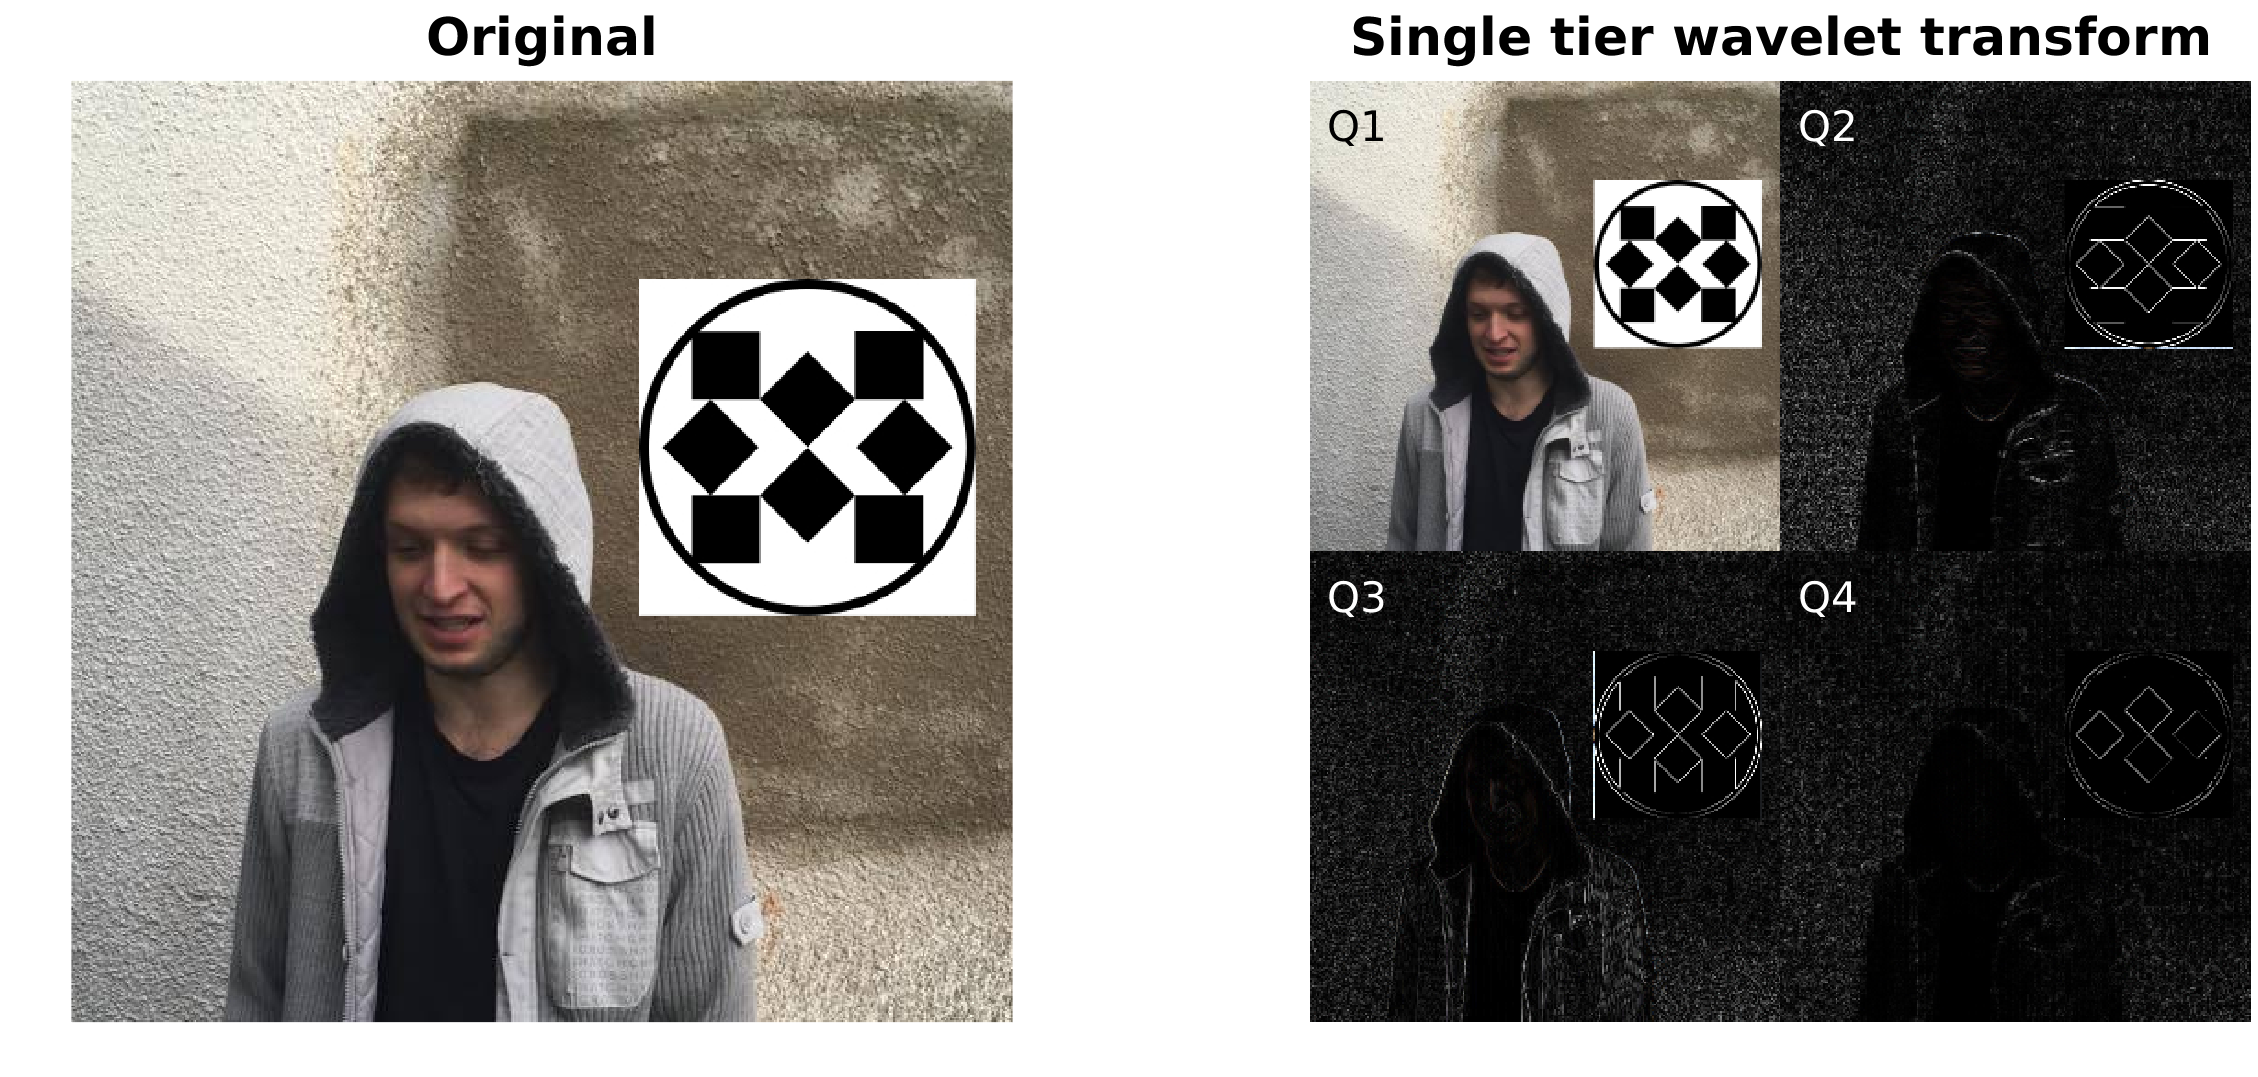
\includegraphics[width=0.75\linewidth, trim={6mm 10mm 4.5mm 3.4mm}, clip]{Chapters/Experimental/wavelet_transform.png}
\caption{ \textbf{Left:} Picture of Rayko Stantchev. \textbf{Right:} Single tier Haar wavelet transform of image on the left. For the transform the wavelet coefficients (quadrants Q2-Q4) have been multiplied by 5 to improve contrast. Large wavelet values are shown as white and indicate regions with strong edges.  \label{fig:wavelet_T}
}
\end{figure}

The next tier of imaging is performed by making a series of Hadamard projection measurements using a fully sampled set of patterns confined to the regions defined by the mask. Here the most common Sylvester Hadamard construction is no longer optimal, as the number of patterns (and therefore pixels) in the Sylvester Hadamard sets are confined to $2^k$, where $k$ is a non-negative integer, while the number of pixels within the next phase is unlikely to equal $2^k$. Therefore we now use the Paley type-$II$ Hadamard construction, which is of more flexible scale, since it can possess a number of patterns equal to $p+1$, where $p$ is a Prime number that is congruent to 3~(mod 4). Therefore we create the smallest Paley type-$II$ Hadamard matrix which can be used to critically or slightly oversample the target area of the object defined by the mask, at twice the resolution of the initial low resolution initial image $I_1$. The fully sampled higher resolution image of the masked regions is once again reconstructed from a weighted sum of the Paley Type-$II$ Hadamard patterns, each weighted by its measured correlation with the object.

Finally, image $I_1$ is upscaled by a factor of 2, and updated to $I_2$ by either replacing those parts of $I_1$ with the higher resolution information, or to make the best use of all measurements, we can combine both low and high resolution measurements by representing all our measurements as a matrix equation as shown in Eqn.~\eqref{eq:y=Ax}, and solving for the image. In the second case, the newly imaged areas are now oversampled, and so a least squares fit provides a level of noise suppression. In the regions that have not been re-sampled at higher resolution we keep our initial low resolution measurements with uniform intensity across each larger scale pixel. Once $I_2$ is obtained, it is used as the input for the single tier Haar wavelet transform and the process is repeated at increasing resolutions. Evidently, as the algorithm progresses, the selection of new regions to image at higher resolutions is likely to be made inside regions that were imaged in the previous phase. This represents the truncation of the Wavelet tree, which is following the assumption that high values of wavelet coefficients at coarse scales are highly correlated with high values at finer scales. This is a reasonable assumption which can be understood by considering that sharp edges are represented by Fourier components across a wide range of frequencies.


